%%%%%%%%%%%%%%%%%%%%%%%%%%%%%%%%%%%%%%%%%%%%%%%%%%%%%%%%%%
\section{\label{sec:Results}Results}
%%%%%%%%%%%%%%%%%%%%%%%%%%%%%%%%%%%%%%%%%%%%%%%%%%%%%%%%%%

In this section, we present our main results for sterile neutrino Dark Matter. However, before discussing the sterile neutrinos themselves, it is very useful to understand the evolution of the singlet scalar in the early Universe, which will make many of our results much easier to grasp.

So let us, just for a moment, assume that the scalar is stable and understand what happens to it. As we had already mentioned, the scalar can either freeze in or freeze out in the early Universe, depending on its interaction strength $\lambda$. We have illustrated all the different cases in Fig.~\ref{fig:interaction_rates}, where we display the ratio between interaction rates $\Gamma_{\rm int}$ of the singlet scalar and the Universe's expansion rate $H$, as functions of the time parameter $r=m_h/T$. The interaction rates $\Gamma_{\rm int}$ are computed using all diagrams available in the different regimes, cf.\ Sec.~\ref{sec:QualitativeDiscussion}, which depending on the processes may receive contributions from different scattering or decay diagrams. As can be concluded from Tab.~\ref{tab:RegimesFeynman}, all diagrams are proportional to $\lambda$, which is why the evolution of the ratio $\Gamma_{\rm int}/H$ with $r$ looks identical for every plot in Fig.~\ref{fig:interaction_rates}, up to a rescaling. However, it is an important information whether $\Gamma_{\rm int}/H < 1$, in which case the scalar freezes in, or whether $\Gamma_{\rm int}/H>1$ and falls off only later on, in which case the scalar first thermalises and then freezes out.

\begin{figure}[t]
\begin{tabular}{lcr}\hspace{-1cm}
 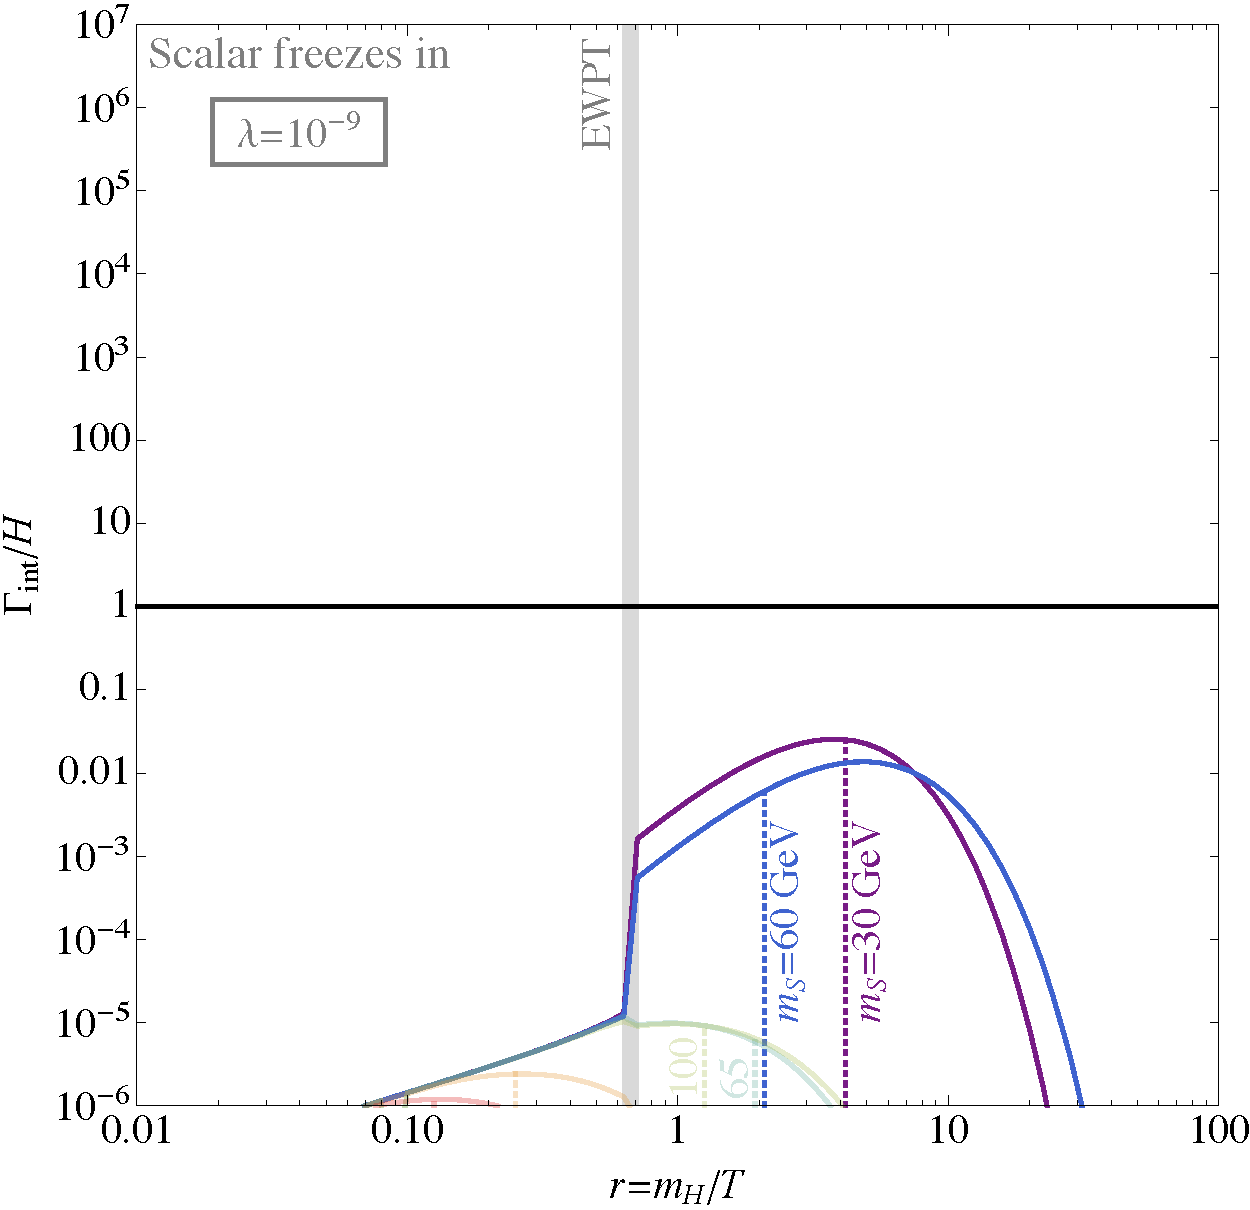
\includegraphics[width=5.5cm]{figures/interactions_FreezeInLight.pdf} & 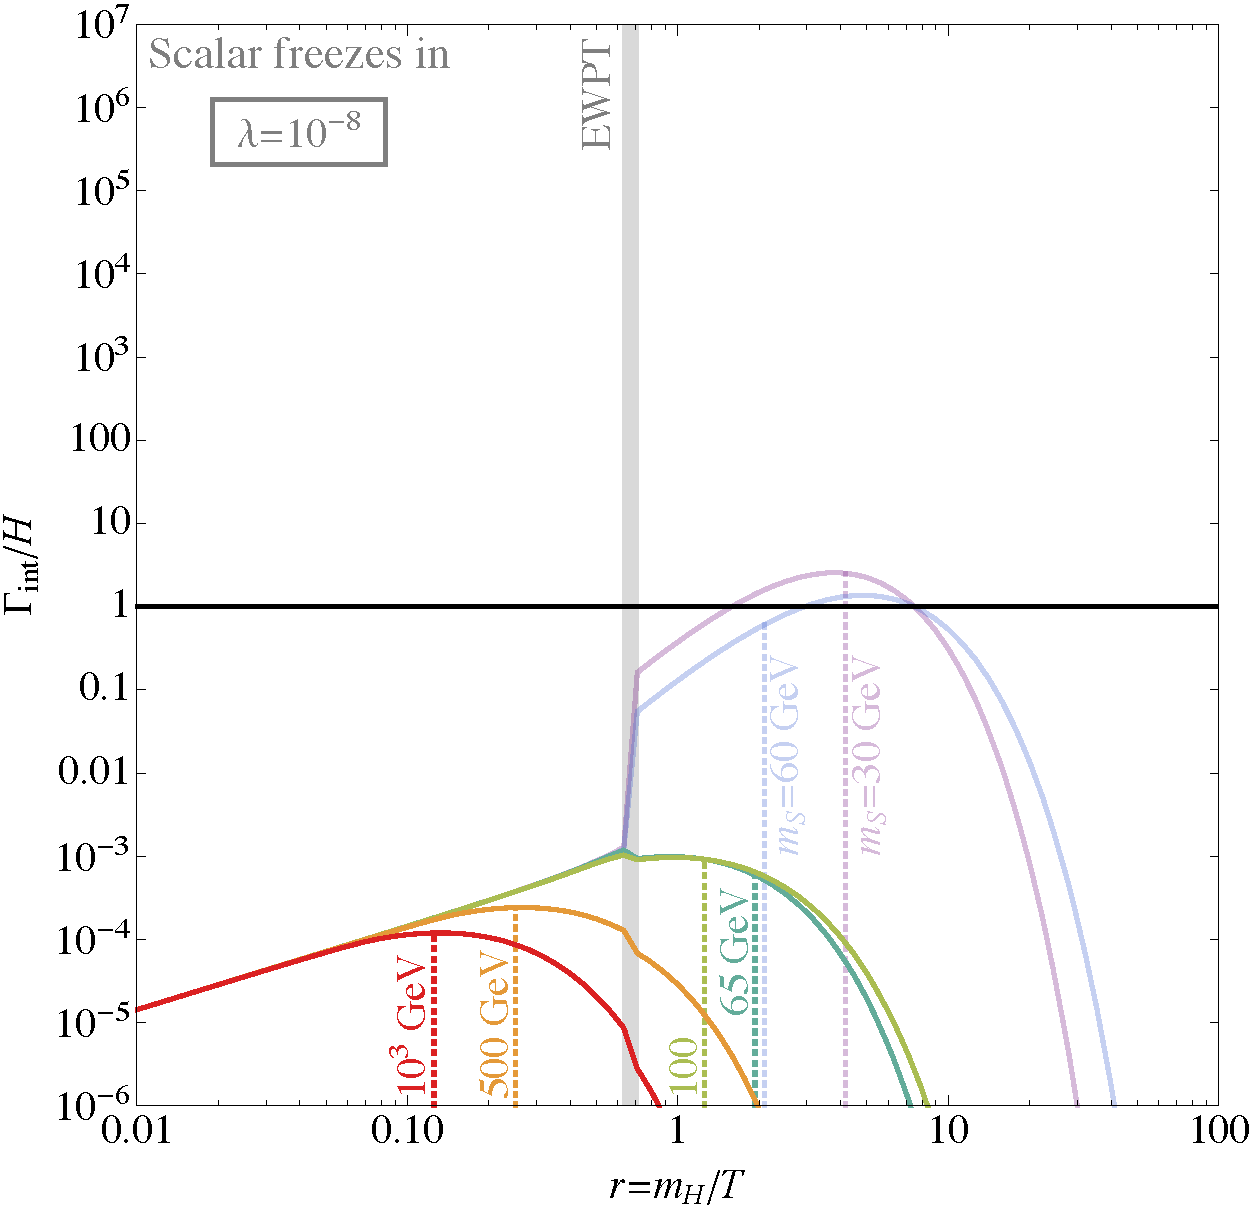
\includegraphics[width=5.5cm]{figures/interactions_FreezeInHeavy.pdf} & 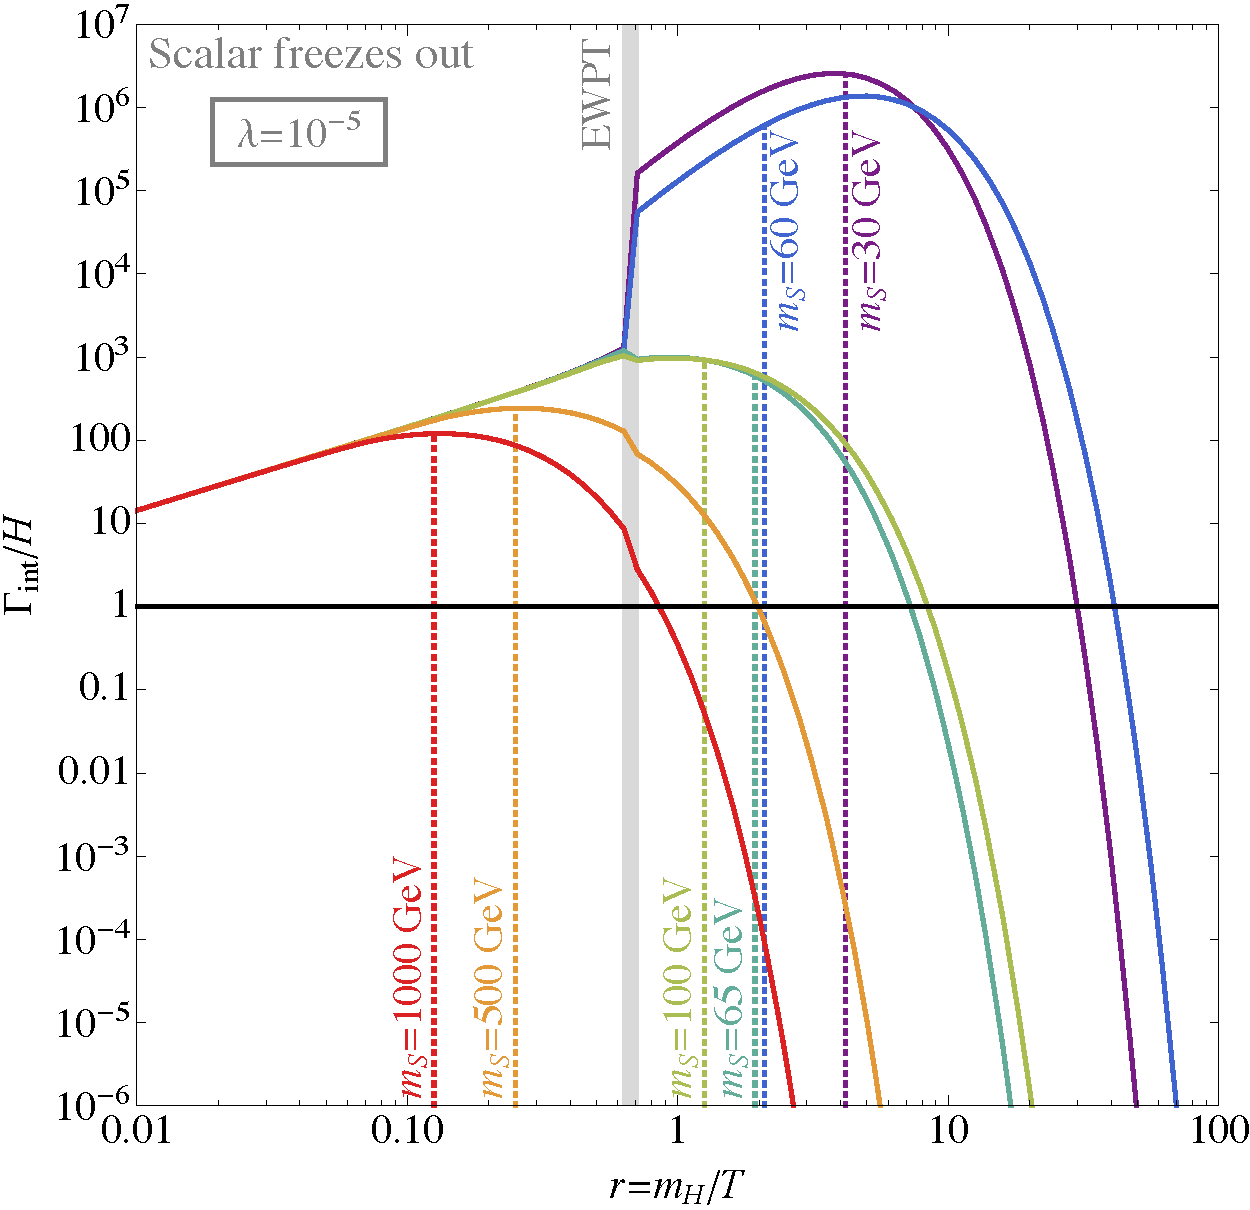
\includegraphics[width=5.5cm]{figures/interactions_FreezeOut.pdf}
\end{tabular}
\caption{\label{fig:interaction_rates}Interaction rates $\Gamma_{\rm int}$ compared to the Universe's expansion rate $H$, as functions of the time parameter $r=m_h/T$. We illustrate two freeze-in cases -- depending on the scalar mass we show either $\lambda=10^{-9}$ (\emph{left}) or $\lambda=10^{-8}$ (\emph{center}) -- as well as one freeze-out case, with $\lambda=10^{-5}$ (\emph{right}). Notably, in the latter, all scalars undergo a \emph{cold} freeze-out a temperatures within $[m_S/20, m_S/4]$, which explicitly proves that it is a good approximation to consider the scalar to be at rest at the point of freeze-out~\cite{Merle:2014xpa}, contrary to the claim made in~\cite{Bezrukov:2014qda}.}
\end{figure}

\paragraph{Freeze-in} Let us start with the freeze-in case. This regime does depend somewhat sensitively on the scalar mass, which is why we have in Fig.~\ref{fig:interaction_rates} depicted the two cases of $\lambda=10^{-9}$ (\emph{left panel}: for $m_S = 30,~60$~GeV) and $\lambda=10^{-8}$ (\emph{central panel}: for $m_S = 65,~100,~500,~1000$~GeV). In all cases, we can clearly see that the scalars are always far from equilibrium.\footnote{In the central plot in Fig.~\ref{fig:interaction_rates}, one can also see the curves for $m_S = 30,~60$~GeV in light colours, which cases apparently can thermalise after a while. This would then lead to an ``overabundance'', at least for this part of the parameter space, which will later also be visible in our main plots -- the sterile neutrinos would need to be so light in order to compensate for the massive number density produced that they are already excluded by several bounds.} We can furthermore see the change in the interaction rates due to the new diagrams available after the EWPT. In particular for very small scalar masses, $m_S = 30$ or $60$~GeV, we can see that the interaction rate jumps up by some two orders of magnitude. This is because for such small masses the Higgs decay $h \to S S$ is available, which is the dominant contribution as noted in Ref.~\cite{Adulpravitchai:2014xna}. For larger scalar masses, in turn, there is hardly any difference visible (if at all, the interaction rates seem to decrease a little); however, the main reason is that larger scalar masses are thermally suppressed at this late stage, as most clearly visible for the largest scalar masses of $m_S = 500$ or $1000$~GeV. But even for medium-scale masses of $m_S = 65$ or $100$~GeV, a small drop in the rate is visible. This is in parts due to kinematics, since the $W$-, $Z$-, and Higgs bosons as well as the top quark are already thermally suppressed at this stage, cf.\ diagrams in Tab.~\ref{tab:RegimesFeynman}, but it happens also because of the different structures of the diagrams involved. In any case, the freeze-in of the scalar ceases at a temperature that is roughly equal to its mass, and indeed all interaction rates start to drop shortly after (or even before) $T = m_S$ is reached. A larger coupling $\lambda$ translates into a larger number density, as expected.

\paragraph{Freeze-out} For the larger coupling, $\lambda=10^{-5}$, scalars of all masses equilibrate. As visible in the \emph{right panel} of Fig.~\ref{fig:interaction_rates}, all interaction rates are larger than the expansion rate already for very early times. As long as the scalars are equilibrated, the actual interaction rate does not matter much. However, a boost in the rate -- as due to the EWPT for $m_S = 30$ and $60$~GeV -- can ``delay'' the freeze-out. This is particularly visible for a $m_S = 60$~GeV, which freezes out at $r \approx 41$ (or at $T\approx m_S/20$), and thus even later than the scalar with $m_S = 30$~GeV, for which freeze-out happens at $r\approx 30$ (or $T\approx m_S/7$). Thus, as we will later see to be correct, we can expect a much larger number density of scalars (and hence of sterile neutrinos) for $m_S = 30$~GeV than for $60$~GeV. Similarly, the case of $m_S = 65$~GeV should yield a larger abundance than the one for $m_S = 100$~GeV, which also turns out to be correct.

\paragraph{Sterile neutrinos} Let us now come to sterile neutrinos as DM. In order to include as much information as possible in the figures, without however making them too busy, we illustrate the allowed ranges and all relevant constraints as ``spaghetti plots'' displayed in Figs.~\ref{fig:verysmall_masses}, \ref{fig:small_masses},~\ref{fig:large_masses}. In these plots, we depict the regions in the $\lambda$--$y$ parameter space where the correct DM abundance is met (where only part of the abundance is produced) by the dark coloured solid lines (by the lightly coloured bands), for different values of the sterile neutrino mass: $m_N = 2, 7.1, 20, 50, 100$~keV. To obtain these regions, we have for each combination of the parameters $(\lambda, y, m_S)$ computed the resulting distribution function along the lines described in Sec.~\ref{sec:Technicalities}, and then integrated the result to obtain the DM abundance according to Eq.~\eqref{eq:DMAbundance}.

In addition, we display the TG phase space bound, as explained in Sec.~\ref{sec:Technicalities:Bounds}. The overclosure bound (gray area) marks the part of the parameter space where we would obtain overclosure of the Universe even for the minimum sterile neutrino mass of $0.5$~keV.

We also display the model-dependent bounds, which only hold in the most minimal setting, cf.\ Sec.~\ref{sec:Technicalities:Bounds}. While they may not even exist in more involved settings, they do serve the purpose of representing the \emph{maximal} effect collider-related bounds could possibly have. To indicate some numbers, the effect of the unitarity bound, Eq.~\eqref{eq:PerturbativeUnitarity2}, for a scalar mass 100~GeV is that the Yukawa coupling $y$ has to be smaller than about $8.2\cdot 10^{-8}$ [$2.9\cdot 10^{-7}$, $8.2\cdot 10^{-7}$] for $m_N = 2$~keV [$7.1$~keV, $20$~keV], in very good agreement with Figs.~\ref{fig:verysmall_masses}, \ref{fig:small_masses},~\ref{fig:large_masses}. For a scalar mass of 1000~GeV, these bounds get stronger by a factor of roughly~10.  The $W$-boson mass correction, Eq.~\eqref{eq:W-mass-bound}, is somewhat more subtle, since the scalar mixing angle $\alpha$ depends on the Higgs portal $\lambda$ which in turn influences the DM abundance and is thus related non-trivially to the Yukawa coupling $y$ and $m_N$. As discussed, these bounds do only exist in the most minimal model, which is why we have marked them by thin dashed lines (see areas left of the TG bound and down in the lower right corners). For some cases, they are even off the plot.

The main bound however arises from structure formation, where we take into account the two Lyman-$\alpha$ bounds derived in Ref.~\cite{Markovic:2013iza} and perform the half-mode analysis described in Sec.~\ref{sec:Technicalities:Bounds} to determine whether a given distribution function is consistent with the data, or not. We have for each scalar mass $m_S$ numerically computed the linear power spectrum for each pair $(\lambda, y)$. Reproducing the correct abundance results in a condition on the sterile neutrino mass $m_N$, so that every point with the correct abundance can be characterised by a point $(m_S, \lambda, y, m_N)$ in the parameter space. Depending on which Lyman-$\alpha$ bound we used, we have in our plots marked the following regions:
\begin{itemize}

\item \textcolor{red}{\bf forbidden}: If the upper half of the squared transfer function is forbidden by both the conservative and restrictive Lyman-$\alpha$ bounds, the respective point is \textcolor{red}{\bf red}.

\item \textcolor{purple}{\bf constrained}: If the upper half of the squared transfer function is only forbidden by the restrictive Lyman-$\alpha$ bound but allowed by the conservative one, the respective point is \textcolor{purple}{\bf purple}.

\item \textcolor{blue}{\bf allowed}: If the upper half of the squared transfer function is allowed by both the conservative and restrictive Lyman-$\alpha$ bounds, the respective point is \textcolor{blue}{\bf blue}.

\end{itemize}
This colour code is slightly reminiscent of the historically grown terms ``hot'', ``warm'', and ``cold'' DM, however, we would like to stress once more that the distributions obtained are \emph{non-thermal}, and one thus \emph{cannot} associate any temperatures with them; see App.~\ref{app:C:FSvsHalfMode} for an explicit counterexample showing that the classification drawn from thermal spectra is bound to fail for non-thermal distributions. Nevertheless it is correct to say that, roughly, the red regime is associated with rather high momenta compared to the DM mass, while the blue one tends to feature smaller momenta. By the light colours, we have indicated regions with a sizable but insufficient abundance for a given mass. Technically, these scenarios correspond to a slightly larger mass which yields the same effect as replacing a fraction of, say 10\% of the Dark Matter by a perfectly cold Dark Matter component. We have checked that this simplified procedure yields correct results up to the level of accuracy limiting analyses using Boltzmann equations anyway.

A final comment on the unavoidable but tiny contribution by Dodelson-Widrow production at temperatures of a few 100~MeV: as had been shown in Ref.~\cite{Merle:2015vzu}, this modification does not only hardly contribute to the abundance for sterile neutrino masses of 4~keV and higher, also the modification of the actual spectrum is completely negligible. Thus, in our plots, there would be no effect visible even if we did take into account the largest modification allowed by data. This may only be different for a sterile neutrino mass of 2~keV, but even then the error by not considering the modification is of about 10\%, which is in practice still negligible. For even smaller masses, the correction could be sizable, but in such cases a mixed scenario would be excluded by structure formation anyway.






%%%%%%%%%%%%%%%%%%%%%%%%%%%%%%%%%%%%%%%%%%%%%%%%%%%%%%%%%%
\subsection{\label{sec:Results_VeryLight}Very light scalars: $\boldsymbol{m_S < m_h/2}$}
%%%%%%%%%%%%%%%%%%%%%%%%%%%%%%%%%%%%%%%%%%%%%%%%%%%%%%%%%%

Let us begin with the case of very light scalar masses, i.e., $m_S < m_h/2$, displayed in Fig.~\ref{fig:verysmall_masses}. As discussed in Sec.~\ref{sec:QualitativeDiscussion}, this leaves us with an interval of roughly $5~{\rm GeV} \lesssim m_S \lesssim 62~{\rm GeV}$. Here, the lower limit arises from the temperature where the relevant interactions are frozen out and/or not efficient anymore, while the upper limit is obtained from $m_h \simeq 125~{\rm GeV}$. Here, depending on the coupling $\lambda$, we may enter different regimes. First of all, for very small couplings $\lambda$, we will be in the FIMP region, i.e., in the left part of the plots. Freeze-in generically is most efficient at temperatures $T$ around the mass $m_S$ of the FIMP, i.e., in regime~III (see Fig.~\ref{fig:RegimeExampleCases} and Tab.~\ref{tab:RegimesFeynman}). Of course the production of scalars has started in regime~I, at high $T$, but in any case -- even with all diagrams of regime~III at work -- the interaction remains feeble. Once the scalar is produced, it decays with a certain lifetime proportional to $y^{-2}$ into sterile neutrinos. Thus, for $y$ large, the decays happen very close to the freeze-in of $S$ and thus the resulting DM particles will be more strongly redshifted and ``cooler''. For too small $y$, in turn, the scalars remain present in the Universe and decay only very late, thus injecting too much energy into the sterile neutrinos and rendering them HDM -- and thus excluded. Notably, as can be seen in the plots, the actual mass of the scalar within the allowed interval does not make much of a difference. The decay rate is proportional to $y^{2} m_S$, such that a larger scalar mass $m_S$ should translate into more red-shift, both because the correct abundance is obtained earlier and and on top of that the decay happens faster. However, for a fixed $y$, the unboosted decay rate also becomes smaller, such that the lifetime effectively increases, leaving less time for the steriles to redshift. To a first approximation, these two effects compensate each other, but of course there will be corrections due to scalars of different masses being boosted more or less (and thus having bigger or smaller lifetmes in the cosmic frame). Apart from these minor effects, the FIMP regions for $m_S=\unit{30}{GeV}$ and $m_S=\unit{60}{GeV}$ appear rather similar, up to a shift in the Higgs portal $\lambda$.

\begin{figure}[t]
\begin{tabular}{lr}\hspace{-1cm}
 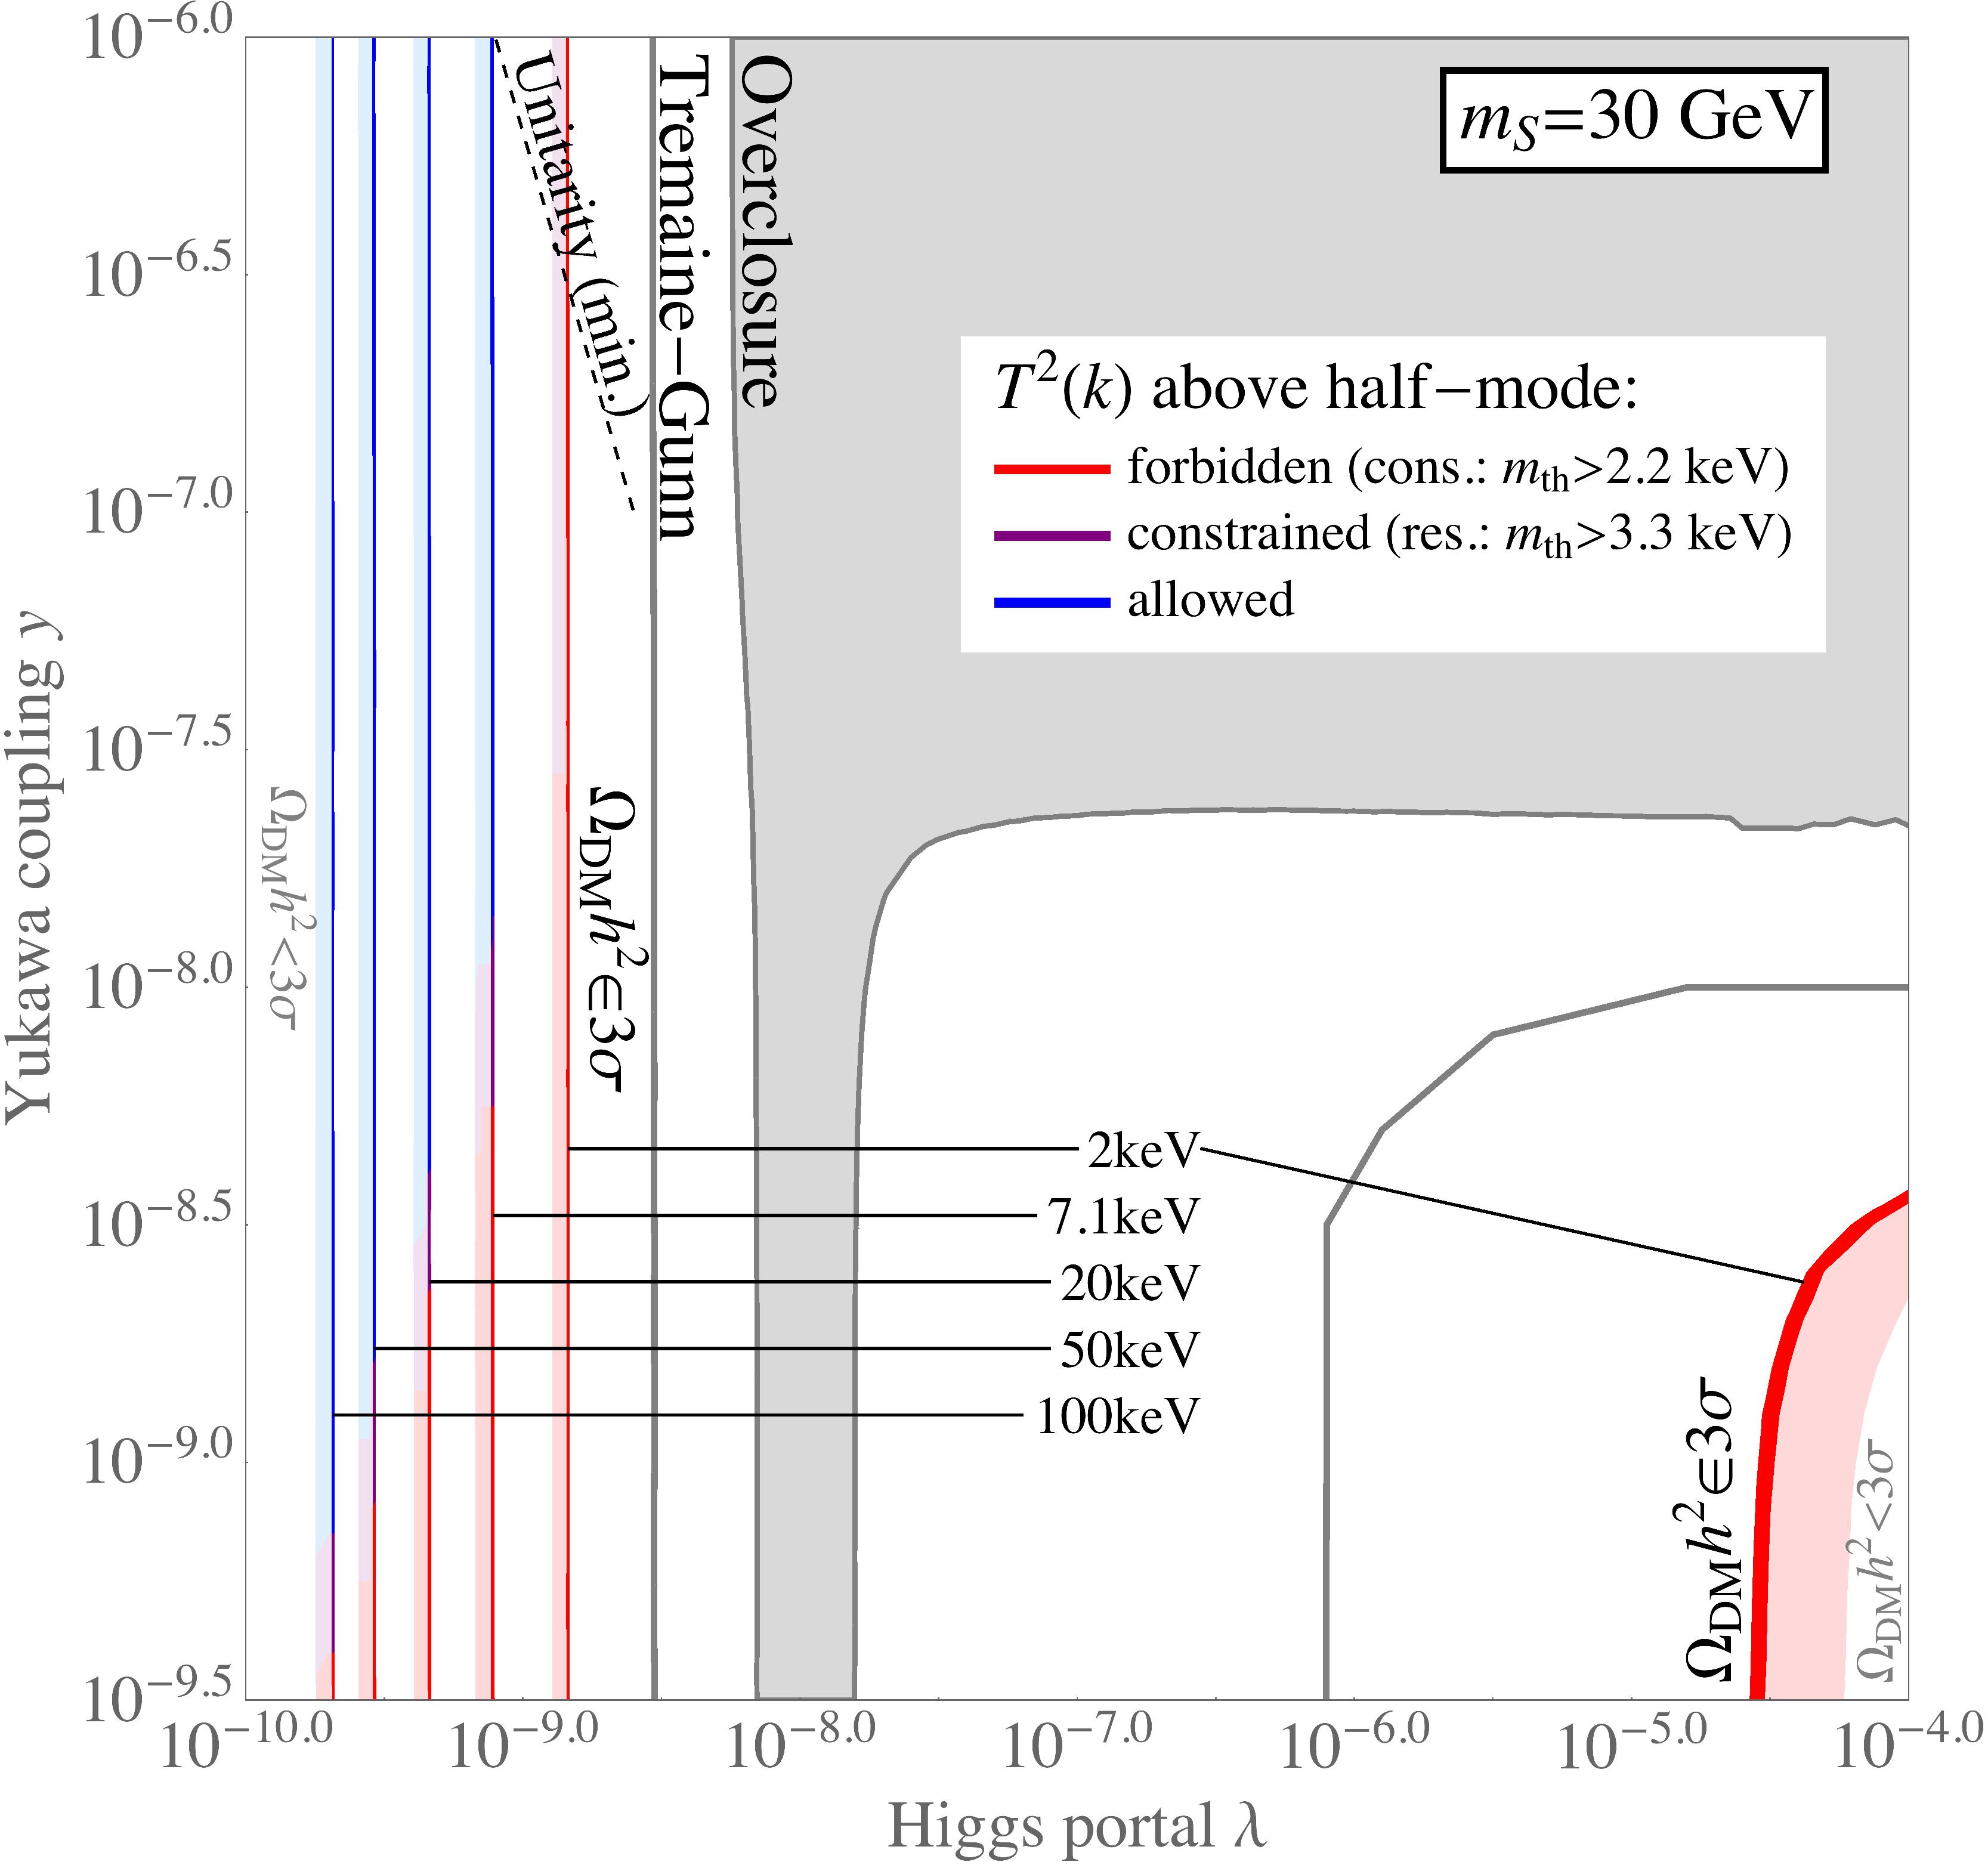
\includegraphics[width=8.3cm]{figures/HalfMode_30_until4.jpeg} & 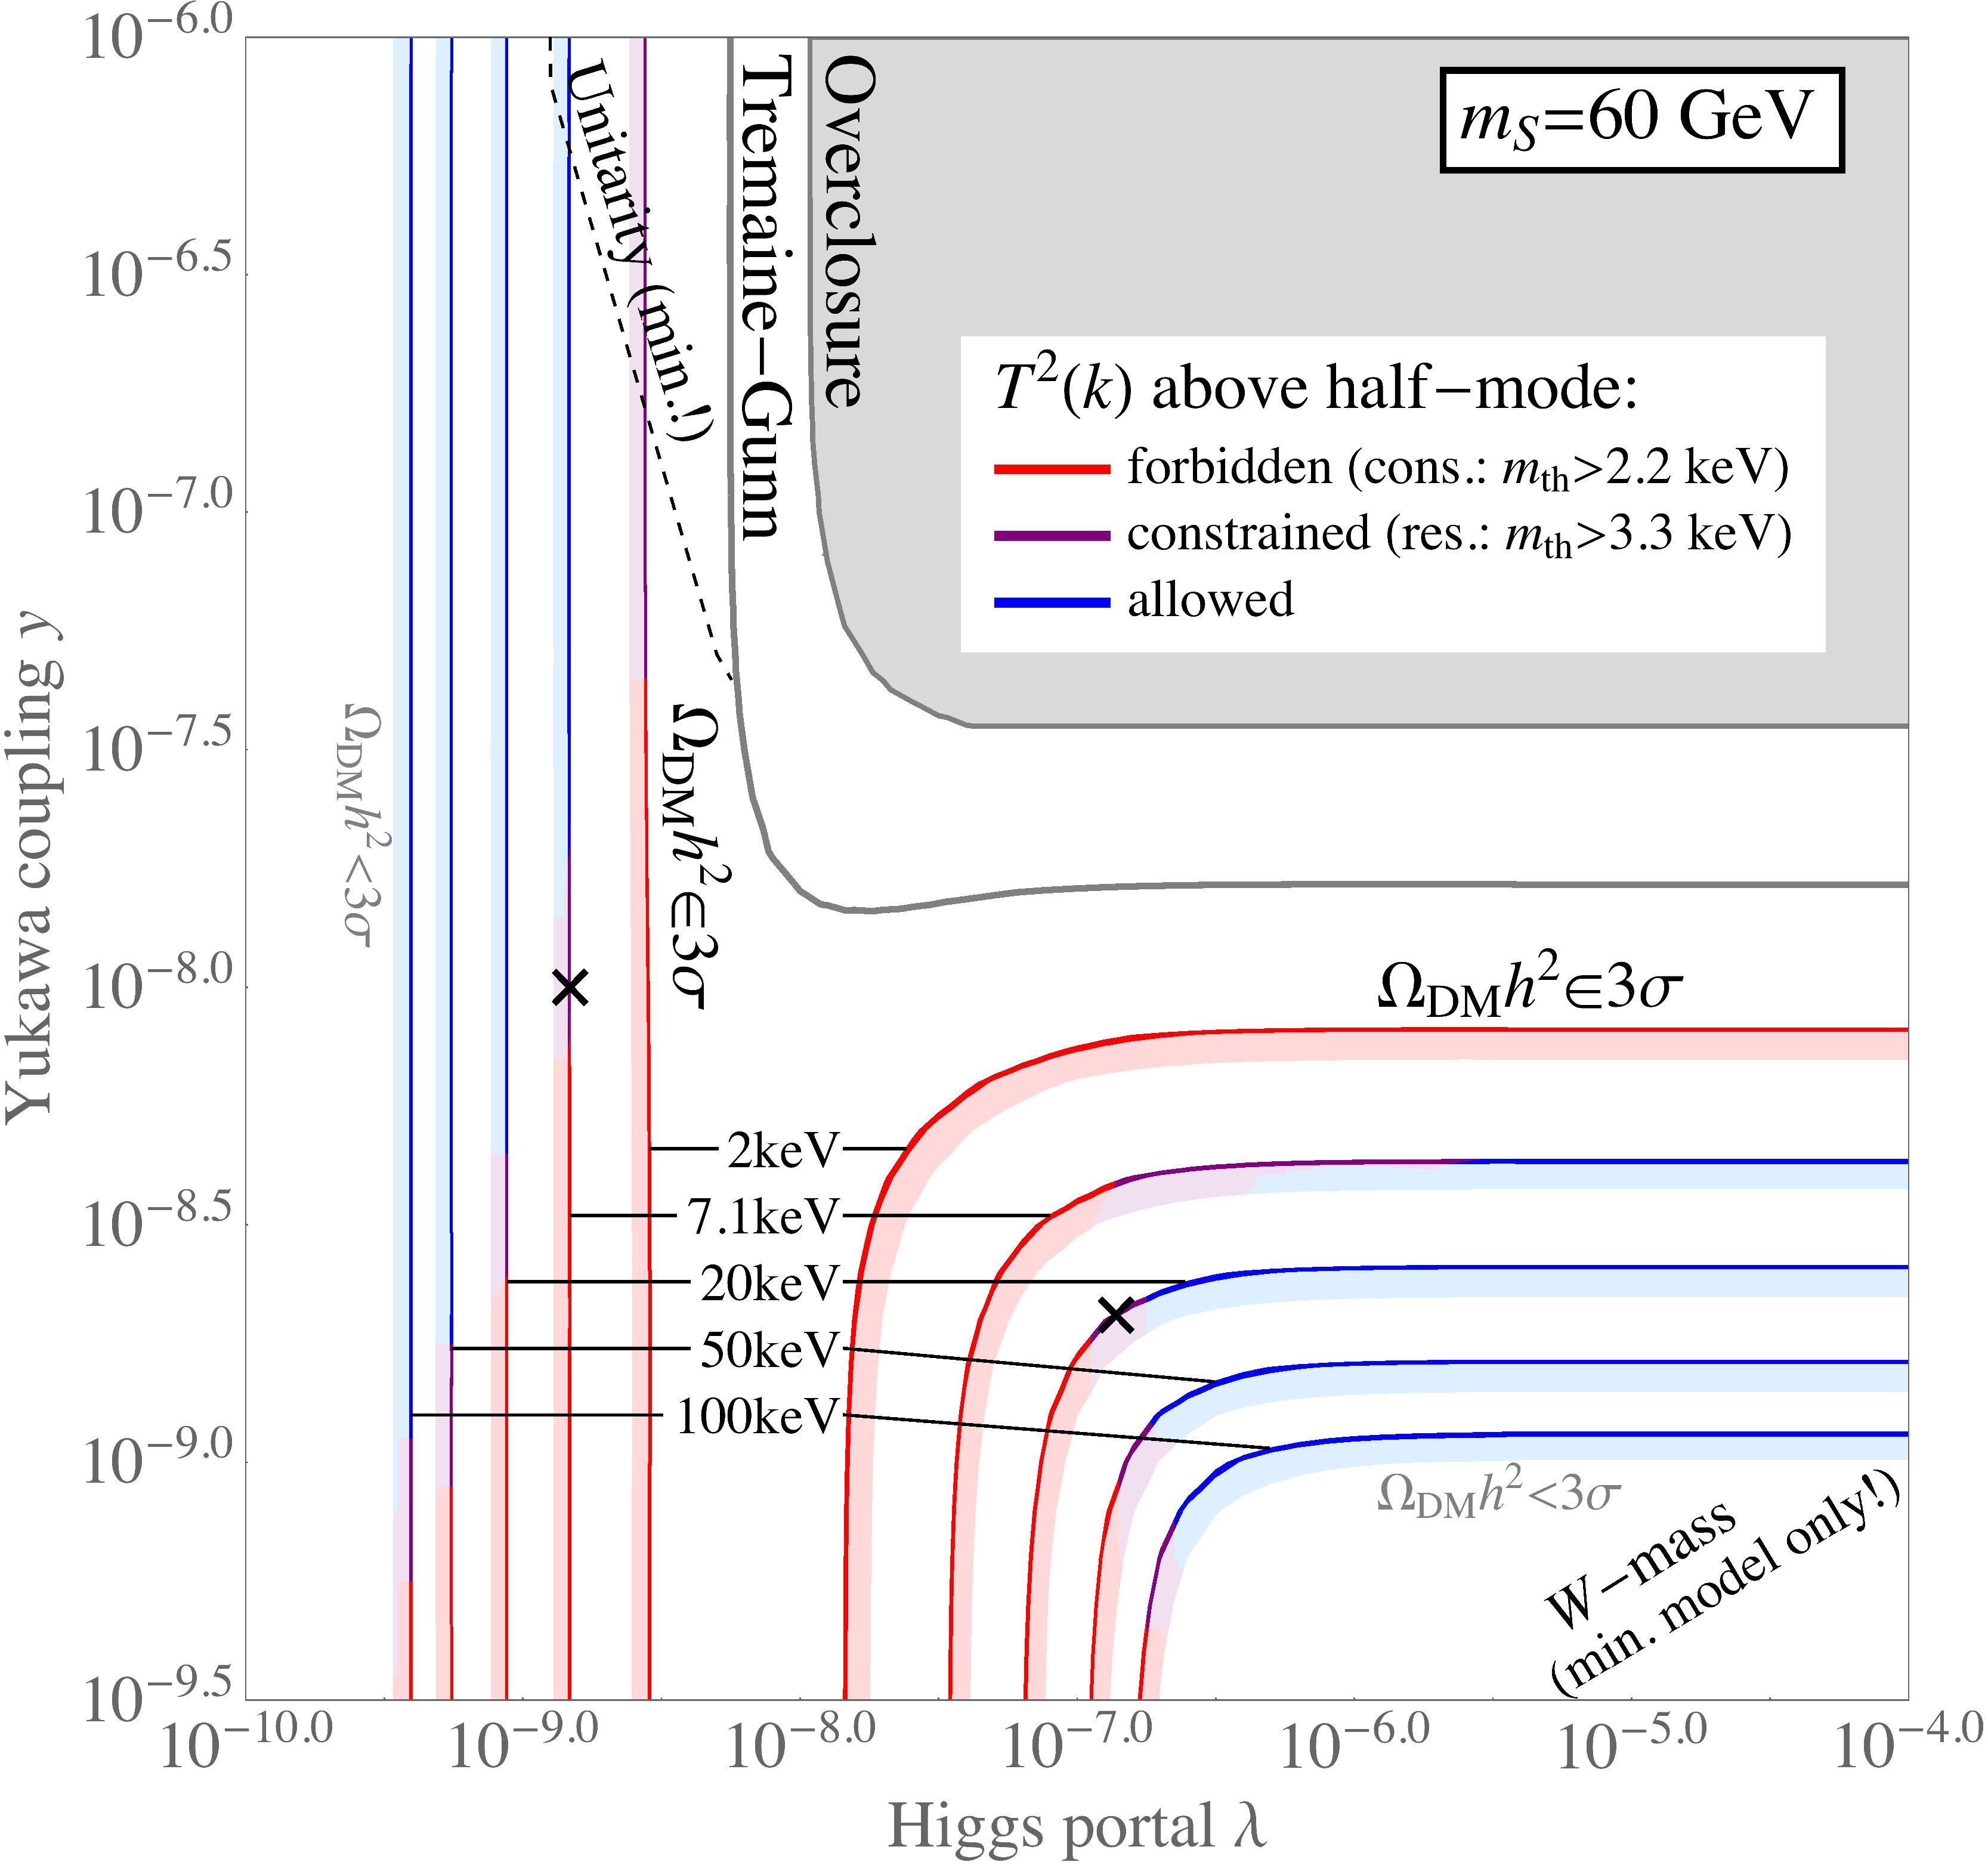
\includegraphics[width=8.3cm]{figures/HalfMode_60_until4.jpeg}
\end{tabular}
\caption{\label{fig:verysmall_masses}Abundance and constraints for small scalar masses, $m_S < m_h/2$. The crosses mark the points displayed explicitly in Fig.~\ref{fig:FIMP_WIMP_60}.}
\end{figure}

On the other hand, for larger values of $\lambda$, the scalar can enter thermal equilibrium and then freeze out, see the lower right regions of the plots. Depending on the exact combination of $(\lambda, y)$, the decay into sterile neutrinos happens while the scalar is in equilibrium (horizontal part of the isoabundance-lines -- which is independent of $\lambda$ from a certain value on), after freeze-out (vertical part -- which is similar to freeze-in in the sense that the scalars cool down before their decay and thus ``forget'' about their cosmological history for a long enough lifetime or small enough coupling $y$), or in between (kink-region -- where a strong dependence on both $\lambda$ and $y$ is present). For this part of the plot, the question of whether there is at all any allowed region depends strongly on $m_S$. This observation can be understood by realising that the scalar freezes out earlier and thus with a much larger abundance for $m_S = 30$~GeV, which is due to the dependence of the interaction rates on the scalar masses. Hence, given many more scalars than for $m_S = 60$~GeV, a too large abundance can only be avoided for sufficiently small sterile neutrino masses -- which is why only one strip is visible in the lower right corner of the left plot, and this one is forbidden by structure formation due to the small DM mass favouring a ``hotter'' spectrum, i.e., with a stronger tendency for large momenta.

\begin{figure}[t!]
\begin{tabular}{cc}
 \hspace{-1cm}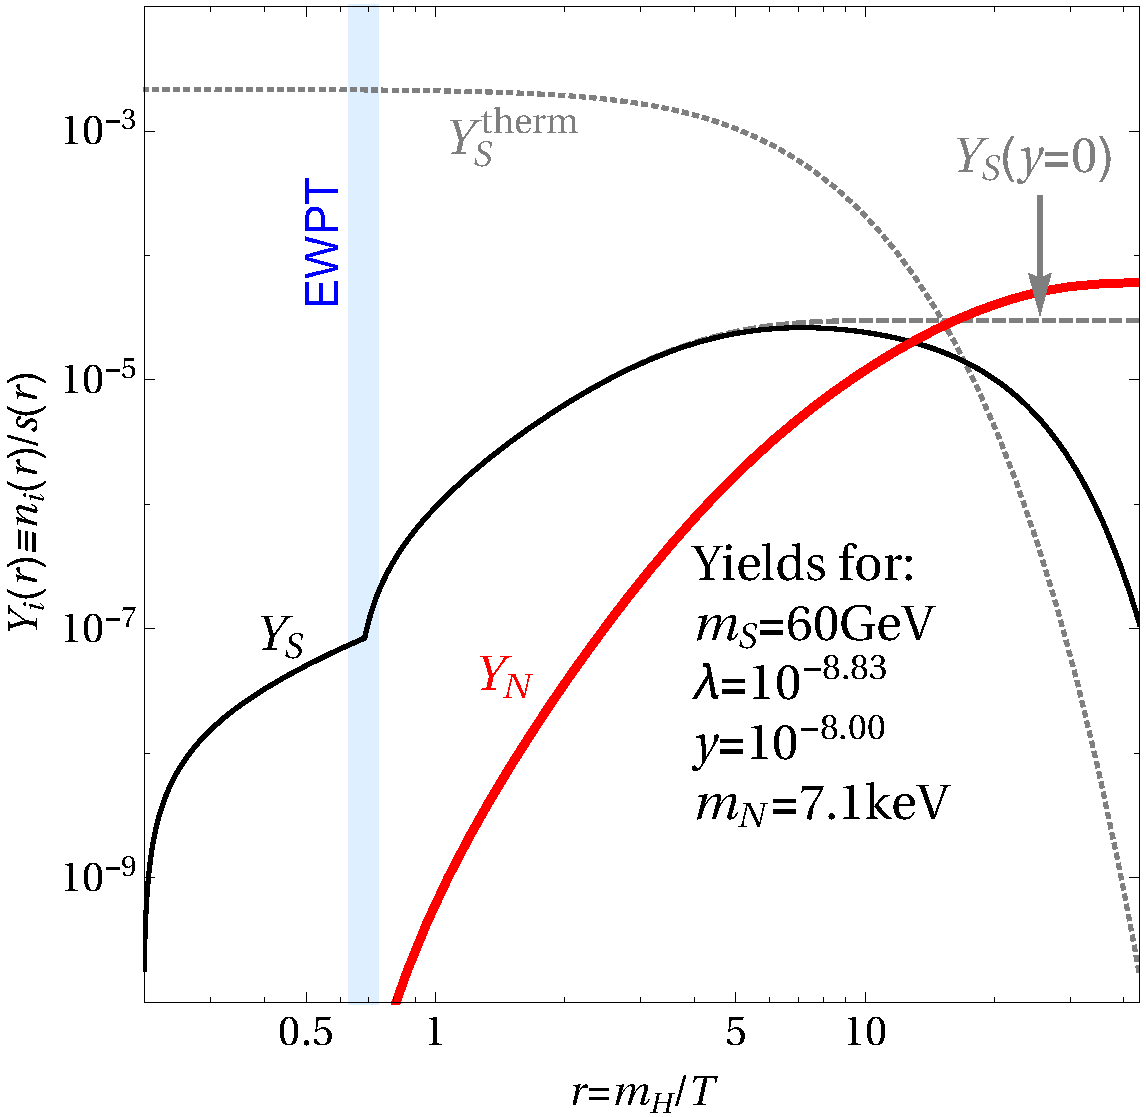
\includegraphics[width=7.9cm]{figures/yield60FIMP.pdf} & 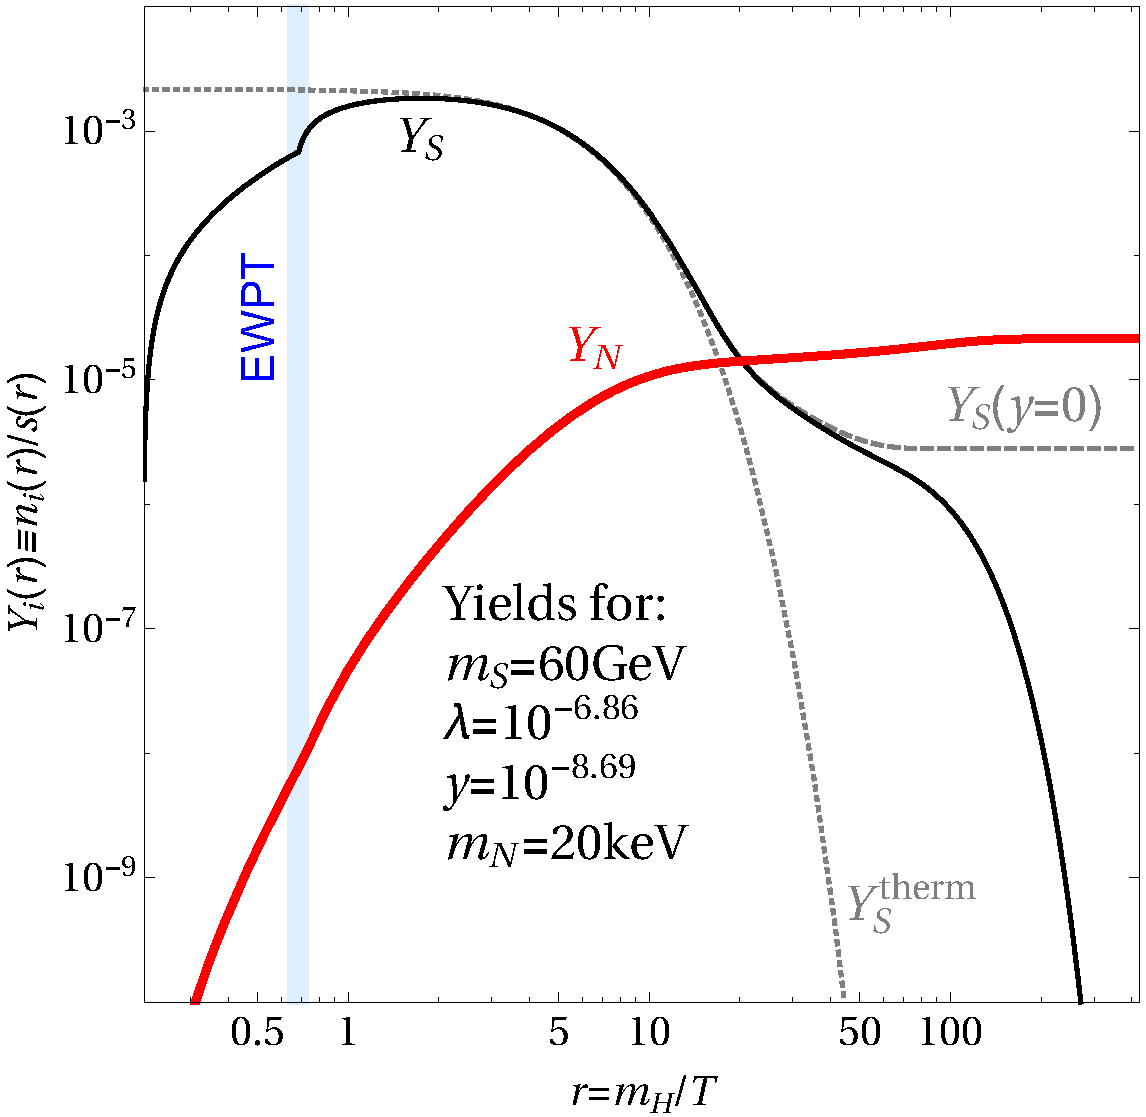
\includegraphics[width=7.9cm]{figures/yield60WIMP.pdf}\\
 \hspace{-1cm}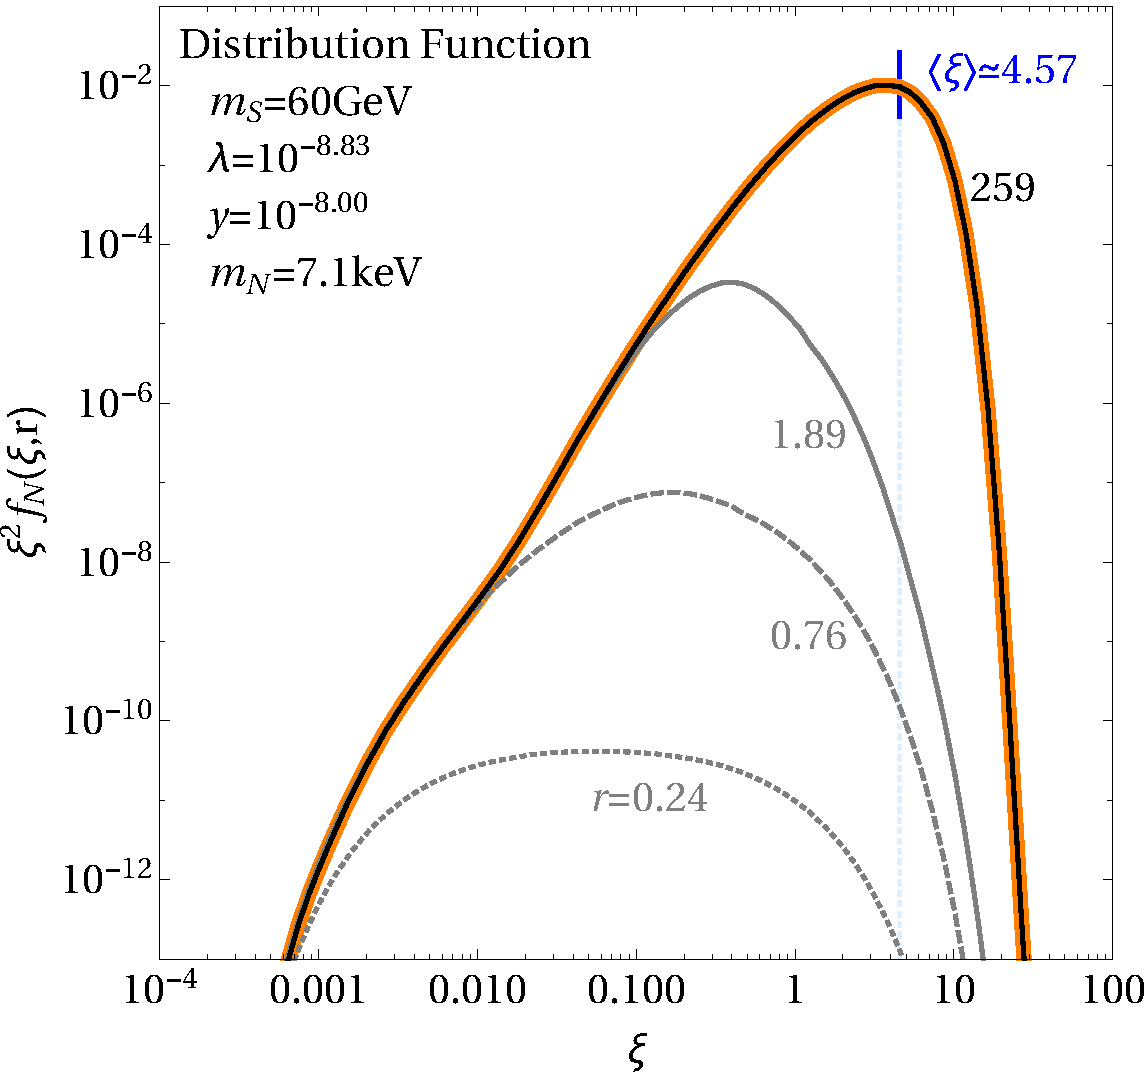
\includegraphics[width=8.3cm]{figures/snapshots60FIMP.pdf} & 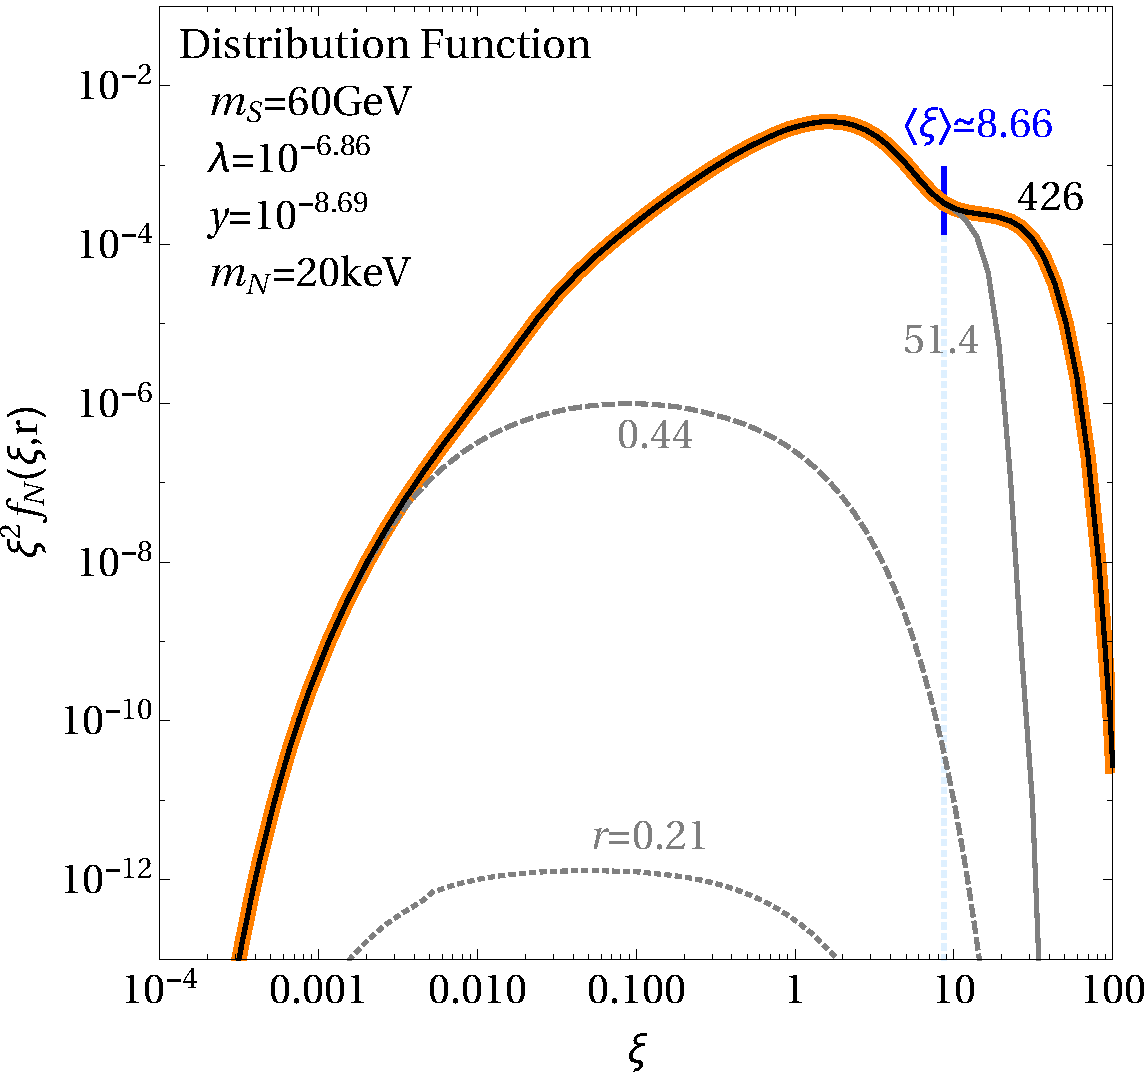
\includegraphics[width=8.3cm]{figures/snapshots60WIMP.pdf}
\end{tabular}
\caption{\label{fig:FIMP_WIMP_60}Example evolutions of the yield (\emph{top row}) and sterile neutrino distributions (\emph{bottom row}) for a scalar with a mass of $60$~GeV undergoing freeze-in (\emph{left}) or freeze-out (\emph{right}) before decaying into sterile neutrinos, for the two points marked in the right Fig.~\ref{fig:verysmall_masses}.}
\end{figure}

Two representative example evolutions of the yield can be seen in the top row of Fig.~\ref{fig:FIMP_WIMP_60}, both for the scalar freezing in (\emph{left}) or out (\emph{right}), which correspond to the crosses marked in the right Fig.~\ref{fig:verysmall_masses}. If the scalar was stable (gray dashed line), it would compare trivially to the hypothetical equilibrium curve (gray dotted line): as a FIMP (\emph{left}), it would gradually be produced but never reach a thermal abundance before freezing in, while as WIMP (\emph{right}) it would quickly thermalise before freezing out. Once the decay into sterile neutrinos is switched on, the true abundance of the scalar (black solid line) again increases initially but ultimately decreases to zero. Note that, in both plots, one can see the increase in the interaction rate due to the EWPT, cf.\ Fig.~\ref{fig:interaction_rates}. The sterile neutrino abundance (red solid line), in turn, increases until the point where ultimately all scalars available have decayed.

Let us make a quick comparison to the results obtained in Ref.~\cite{Adulpravitchai:2014xna}. Looking at the top two plots in their Fig.~2, which feature the same scalar masses as our top two plots in Fig.~\ref{fig:FIMP_WIMP_60}, our yields look qualitatively very similar except for a missing ``bump'' in the yield of the scalar for temperatures around $10$~GeV, which appears in Ref.~\cite{Adulpravitchai:2014xna} but not in our result. While we cannot explain this feature, we do however have good agreement with the overall abundance obtained in~\cite{Adulpravitchai:2014xna},\footnote{To see this, one has to adjust the pair $(\lambda,y)$ to the case from~\cite{Adulpravitchai:2014xna}, though, taking into account the different normalisation of $\lambda$ in their Eq.~(5) compared to our Eq.~\eqref{eq:ModelLagrangian}.} up to some 20\% difference, which can be attributed to applying different numerical procedures and also due to Ref.~\cite{Adulpravitchai:2014xna} using some approximations such as rate equations assuming a (suppressed) thermal shape.

The evolution of the resulting sterile neutrino distributions for the same two points is displayed in the bottom row of Fig.~\ref{fig:FIMP_WIMP_60}, with all spectra being functions of $\xi = \left( \frac{g_{s}(T_0)}{g_{s}(T)} \right)^{1/3}\;\frac{p}{T}$, cf.\ the second Eq.~\eqref{eq:xi_and_r_definition}. We can see a certain deformation in both curves, although the one on the left (for the scalar being a FIMP), it is probably a small bump rather than an actual double peak. In both cases, these shapes come from two different production phases. In the FIMP case (\emph{left}), the two phases correspond to the production before and after the EWPT, whereas the visible bump for larger $\xi$ for the WIMP case (\emph{right}) rather comes from production while the scalar is still in equilibrium and after its freeze-out, respectively.\footnote{Note that, in the spectrum on the right, a tiny bump stemming from the changes during the EWPT is nevertheless visible at around $\xi \sim 0.03$, thereby implying a third momentum scale. However it is so tiny that it does not have a real influence on the spectrum.}

Finally, in Fig.~\ref{fig:TF_60}, we display the squared transfer functions for the two example points. Glancing at the right Fig.~\ref{fig:verysmall_masses}, we can see that both points lie inside ``purple'' regions, i.e., they are constrained but not excluded by the Lyman-$\alpha$ bounds. According to the procedure detailed in Sec.~\ref{sec:Technicalities:Bounds}, this would imply that the parts of the squared transfer functions with $k \leq k_{1/2}$ should both be consistent with the conservative Lyman-$\alpha$ bound, but inconsistent with the restrictive one. This is just what we can see in Fig.~\ref{fig:TF_60}. It is also visible that, in particular for the FIMP case depicted on the left, the slope of the functions is different from that of the bounds, for which the distributions were thermal by construction. Furthermore, note that the sterile neutrino mass on the left plot, $7.1$~keV, is significantly different from the mass of $2$~keV corresponding to the conservative bound, which originates from the non-thermal shape of the scalar-decay produced DM spectrum. Obviously, according to the left Fig.~\ref{fig:TF_60}, one would classify the case displayed as ``warmer'' than the restrictive bound corresponding to a mass of $3.3$~keV, even though the true DM mass is even larger than that. This is one more reflection of conclusions which do hold for thermal spectra being invalidated once the shape of the momentum distribution function is more complicated. Thus, any ``translation'' of the structure formation properties to a hypothetical spectrum of thermal shape, as attempted for DW-produced sterile neutrinos on several occasions in the literature (e.g.\ Refs.~\cite{Colombi:1995ze,Viel:2013apy,Markovic:2013iza,Abada:2014zra,Popa:2015eta,Bozek:2015bdo,Baur:2015jsy}), must be treated with extreme care and should not be regarded as a precision statement.

\begin{figure}[t]
\begin{tabular}{lr}\hspace{-1cm}
 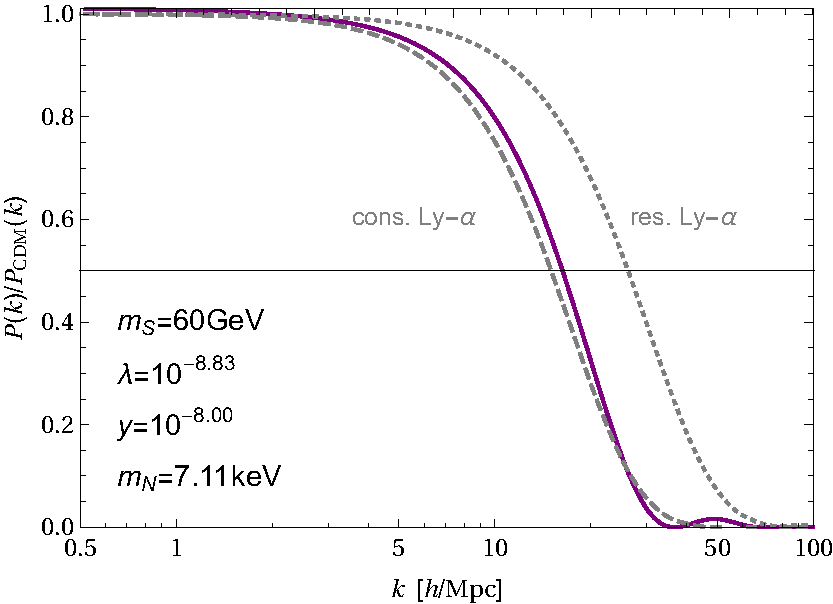
\includegraphics[width=8.3cm]{figures/SquaredTF_mS_60_FIMP.pdf} & 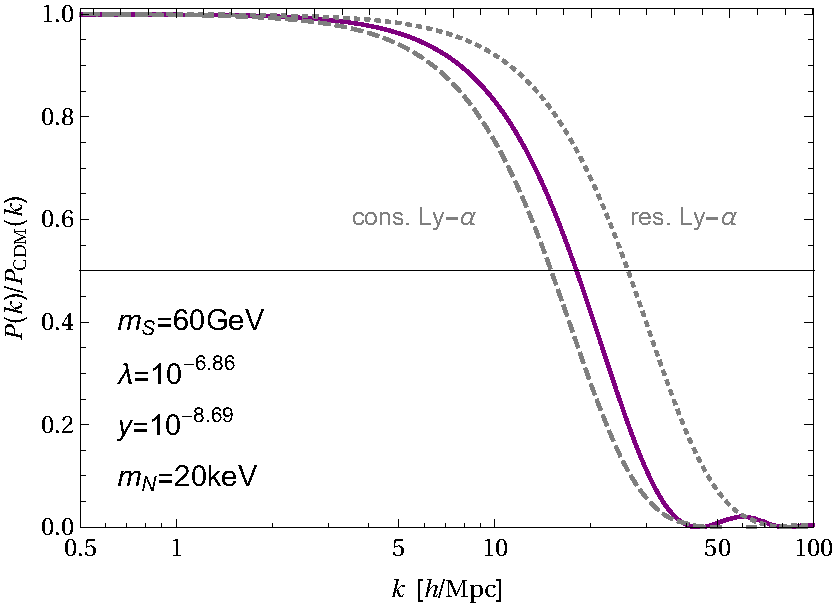
\includegraphics[width=8.3cm]{figures/SquaredTF_mS_60_WIMP.pdf}
\end{tabular}
\caption{\label{fig:TF_60}Example squared transfer functions for a scalar with a mass of $60$~GeV undergoing freeze-in (\emph{left}) or freeze-out (\emph{right}) before decaying into sterile neutrinos, for the two points marked in the right Fig.~\ref{fig:verysmall_masses}.}
\end{figure}

We can also see that, although both of the points that we had explicitly illustrated above fall into the same category in what concerns structure formation, the FIMP case tends to be slightly ``warmer'', i.e., closer to being excluded than the WIMP example. This may come as a small surprise, given that the average momentum of the WIMP-produced sterile neutrino is nearly two-times larger than the FIMP-produced one.\footnote{Note that, while one has to be slightly careful when converting the quantity $\xi$ to a physical momentum, cf.\ Sec.~\ref{sec:Technicalities:BoltzmannEquation-solution}, it can still be used to compare the relative average momenta of two given spectra.} However, when dividing the average momenta by the sterile neutrino masses, hence looking at the average velocities, the factor of nearly two remains present -- just that in this case the FIMP-produced particle yields the larger value.

Looking back at Fig.~\ref{fig:verysmall_masses}, to get a more global picture, it is visible in the freeze-in (\emph{left}) regions that for larger Yukawa couplings $y$ the DM particles get ``colder'' (i.e., shifted to smaller momenta). This is due to the parent particles decaying earlier, thus leaving more time for the DM particles to redshift. Of course, this effect is more pronounced when the DM particles are heavier, see upper left corners of the plots. Interestingly, the unitarity bound would cut off part of that otherwise allowed parameter space (but only if $m_N = y \langle S \rangle$). For the freeze-out (\emph{right}) regions, instead, the case of small Yukawa coupling corresponds to a very late decay, always far after the freeze-out. This leaves the DM particles no time to cool down, so that they will generically be threatened by structure formation. The second limit of large $\lambda$ keeps the scalars in equilibrium for a very long time, so that practically all sterile neutrinos are produced while the scalar is still equilibrated. That leads to a ``colder'' spectrum, because the DM particles have more time to redshift. The turnover, corresponding to the double peak structure observed in Ref.~\cite{Merle:2015oja} for the first time, can be somewhere in between. Depending on the (non-trivial) interplay between the different parameters and in particular on the relative strength of the two peaks, it can be ruled in or out by structure formation.






%%%%%%%%%%%%%%%%%%%%%%%%%%%%%%%%%%%%%%%%%%%%%%%%%%%%%%%%%%
\subsection{\label{sec:Results_Light}Light scalars: $\boldsymbol{m_h/2 < m_S < m_h}$}
%%%%%%%%%%%%%%%%%%%%%%%%%%%%%%%%%%%%%%%%%%%%%%%%%%%%%%%%%%

\begin{figure}[t]
\begin{tabular}{lr}\hspace{-1cm}
 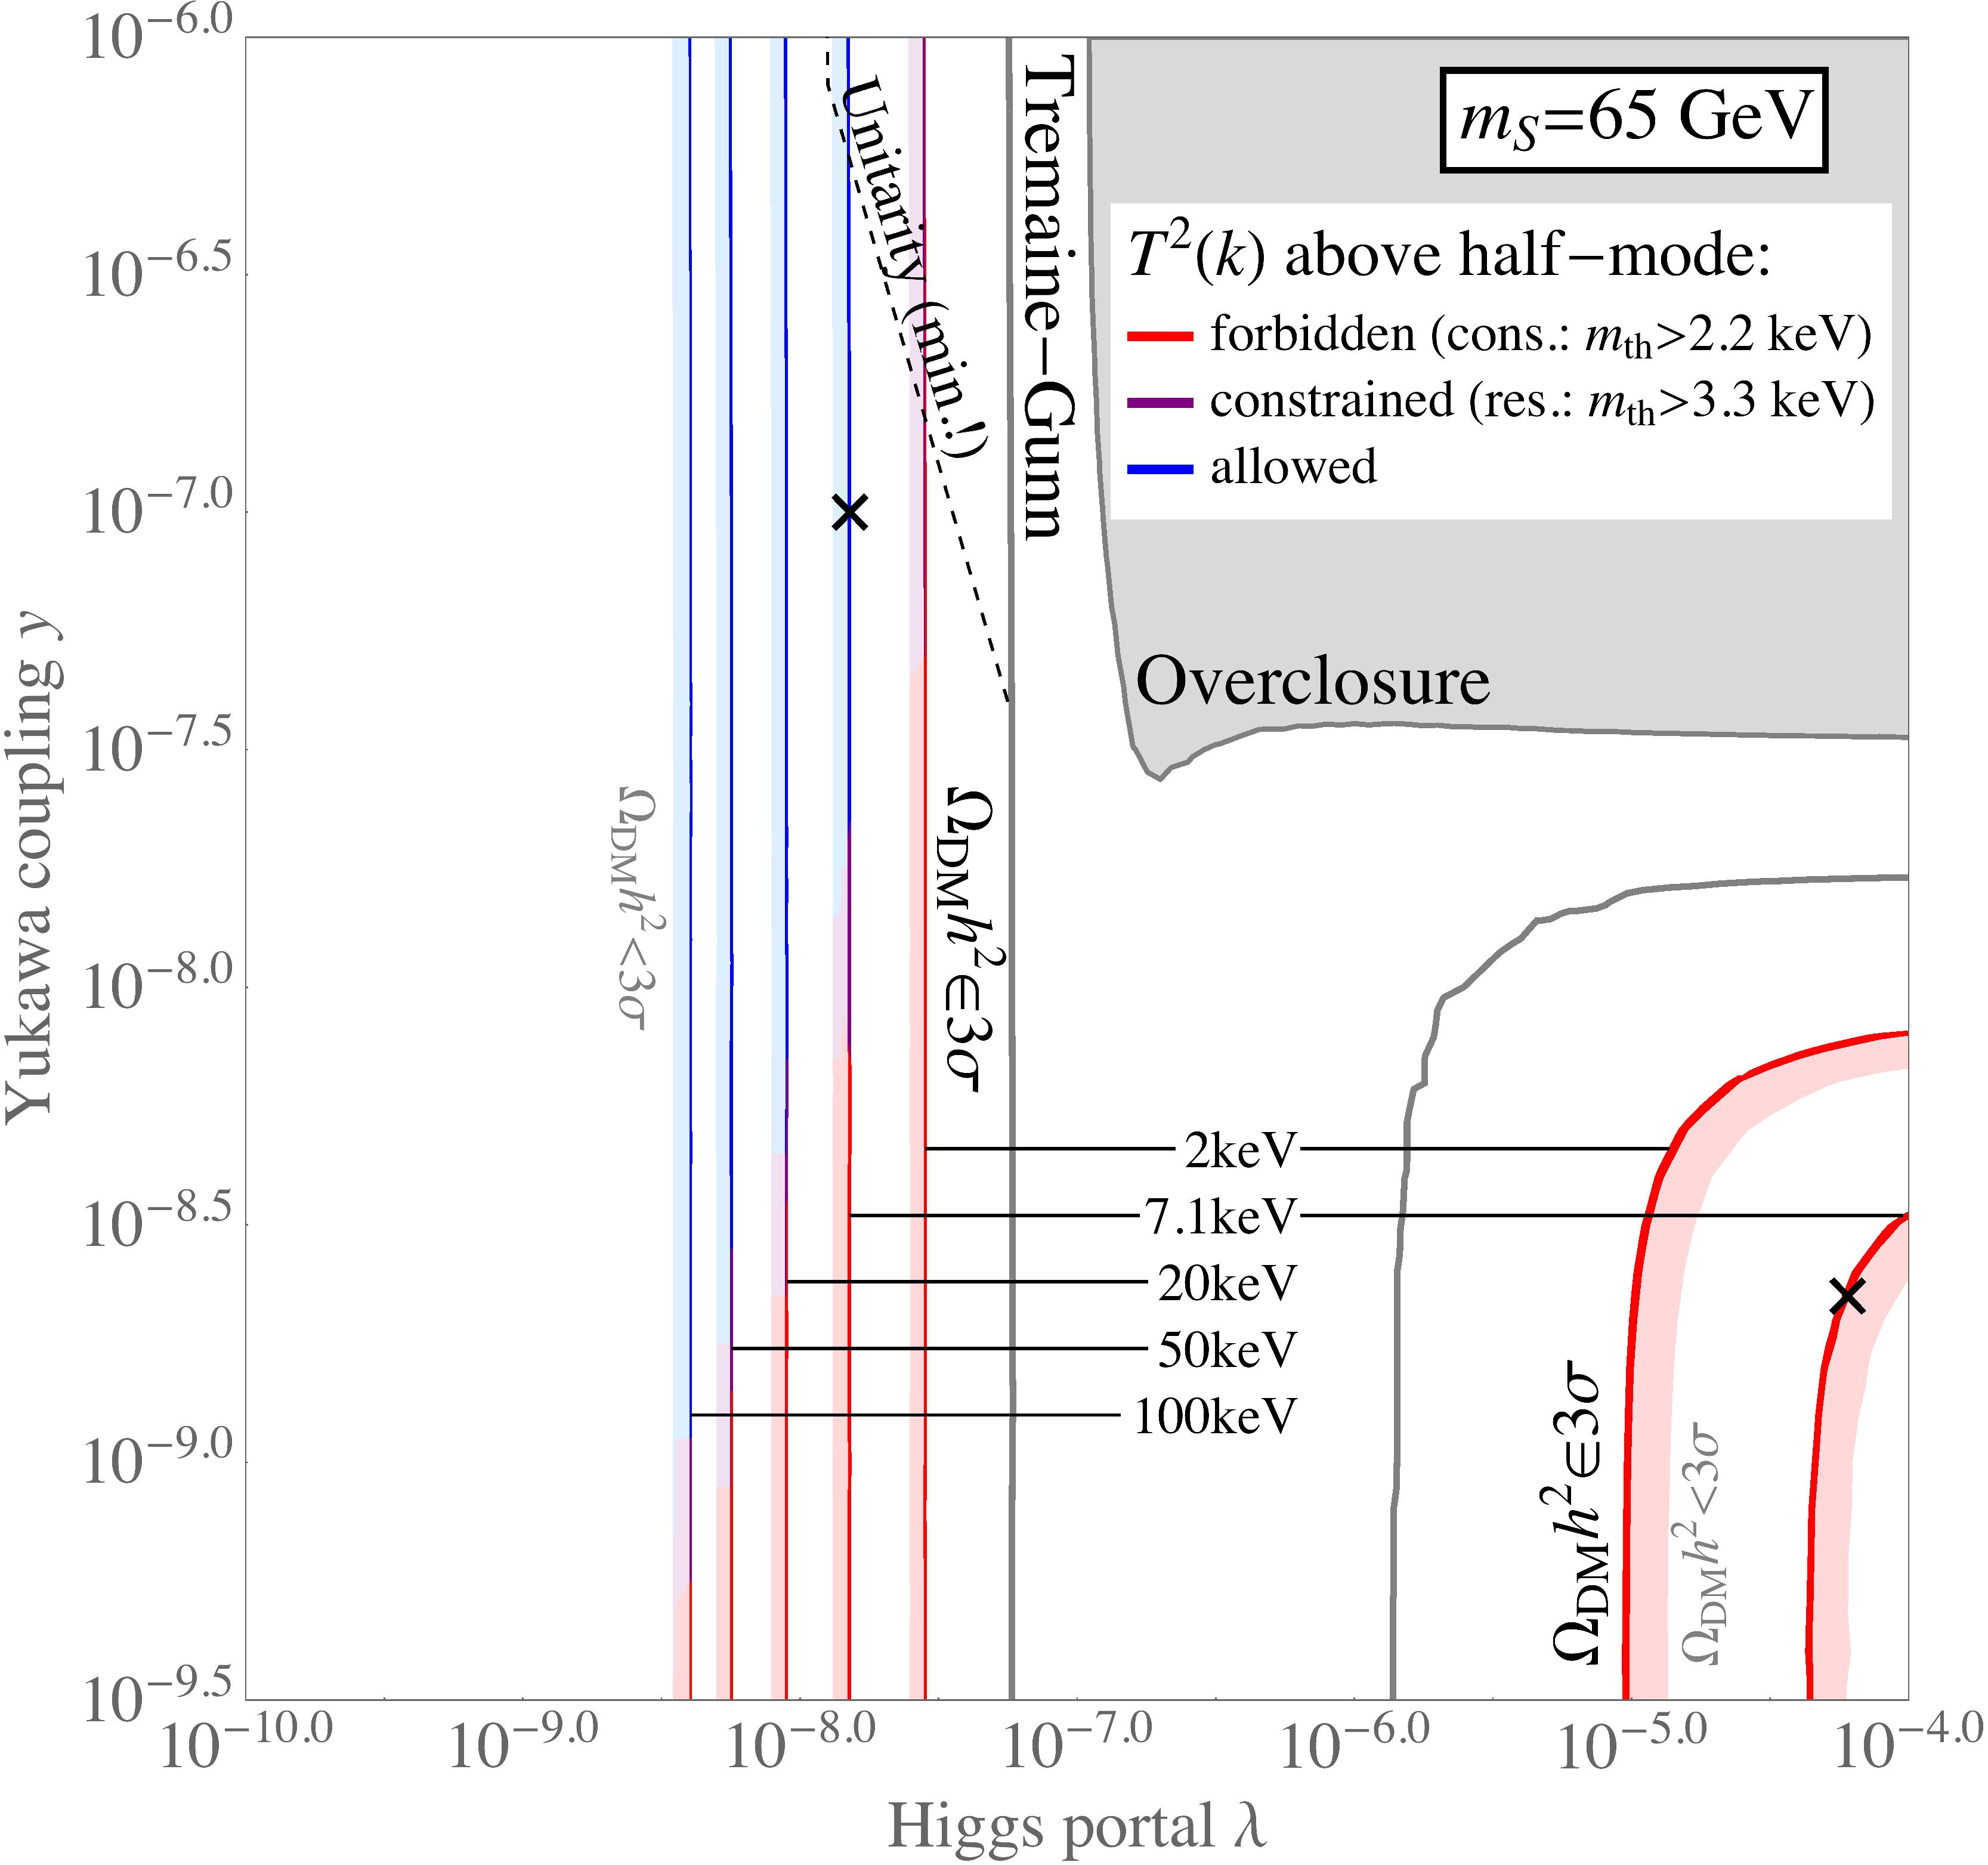
\includegraphics[width=8.3cm]{figures/HalfMode_65_until4.jpeg} & 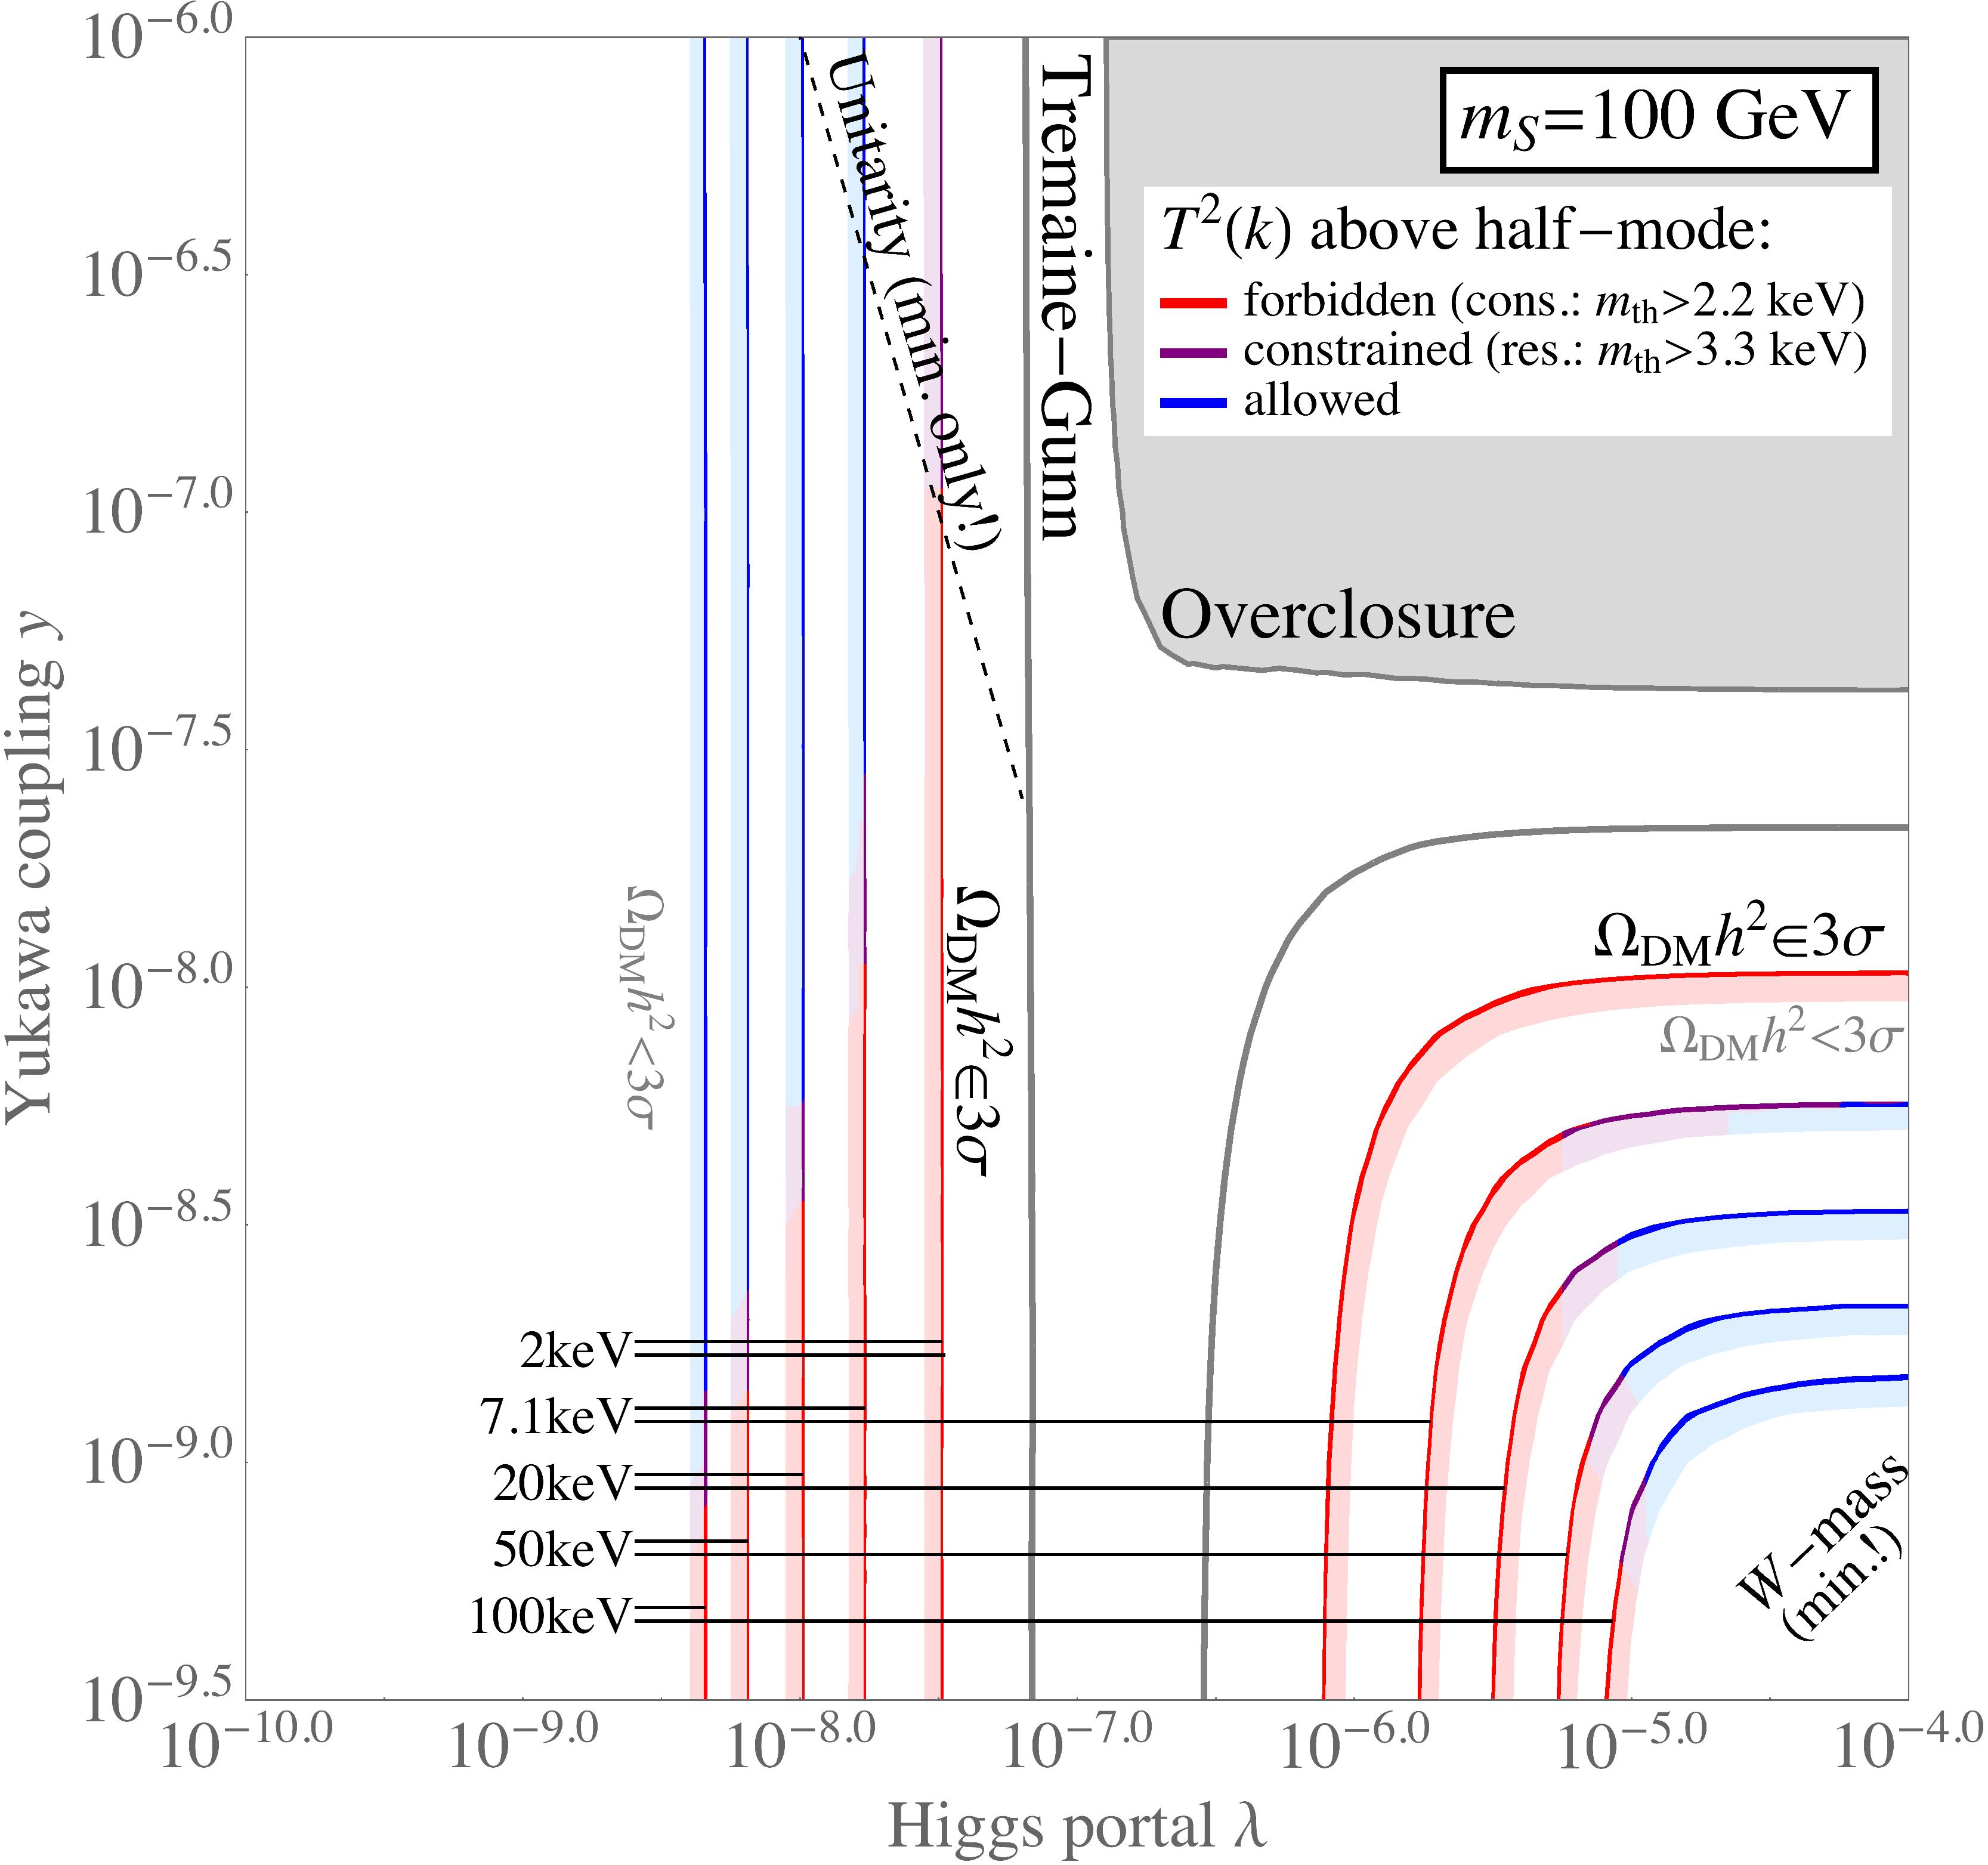
\includegraphics[width=8.3cm]{figures/HalfMode_100_until4.jpeg}
\end{tabular}
\caption{\label{fig:small_masses}Abundance and constraints for intermediate scalar masses, $m_h/2 < m_S < m_h$. The crosses mark the points displayed explicitly in Fig.~\ref{fig:FIMP_WIMP_65}.}
\end{figure}

The next case to be discussed, cf.\ Fig.~\ref{fig:small_masses}, is that of ``light'' scalars, in the sense that their mass is still less than the mass $m_h$ of the Higgs boson, but larger than half the Higgs mass. This corresponds to regime~II in Tab.~\ref{tab:RegimesFeynman} for low temperatures $T$, while the production nevertheless starts at high $T$ and thus in regime~I, cf.\ Fig.~\ref{fig:RegimeExampleCases}. Here, the main characteristic is that, at the EWPT, all of a sudden lots of new channels open up. For the freeze-in case, i.e.\ small $\lambda$, this means that it is easier to produce scalars at a temperature just above their mass, which will result in an increase in their abundance and thus also in that of sterile neutrinos -- however this increase is much less dramatic than for the very light scalars, and hence hardly visible in the plots, due to the Higgs decay into two scalars not anymore being accessible in this mass range. For the freeze-out case, i.e.\ large $\lambda$, this means that the scalars will be kept in equilibrium for a longer time in regime~II, resulting into a large overall number of sterile neutrinos produced while the scalar is still equilibrated.

The spaghetti plots for two different scalar masses, $m_S = 65$ and $100$~GeV, are depicted in Fig.~\ref{fig:small_masses}. At first sight, these plots appear qualitatively similar to those depicted in Fig.~\ref{fig:verysmall_masses}, except for an overall shift towards larger values of $\lambda$. However, an interesting observation is that, for the FIMP case, the spectrum seems to become ``warmer'' when going from $m_S = 65$ to $100$~GeV, while the trend was opposite when going from $m_S = 30$ to $60$~GeV. The reason is that, for the case at hand, Higgs decay does not play a role in the production of the scalar. Instead, many scalars are already produced rather early (see upper left panel of Fig.~\ref{fig:FIMP_WIMP_65}), such that they can indeed decay earlier (and are less boosted), so that in this case a smaller scalar mass results into smaller initial sterile neutrino velocities and this effect dominates the production. 

\begin{figure}[t!]
\begin{tabular}{cc}
 \hspace{-1cm}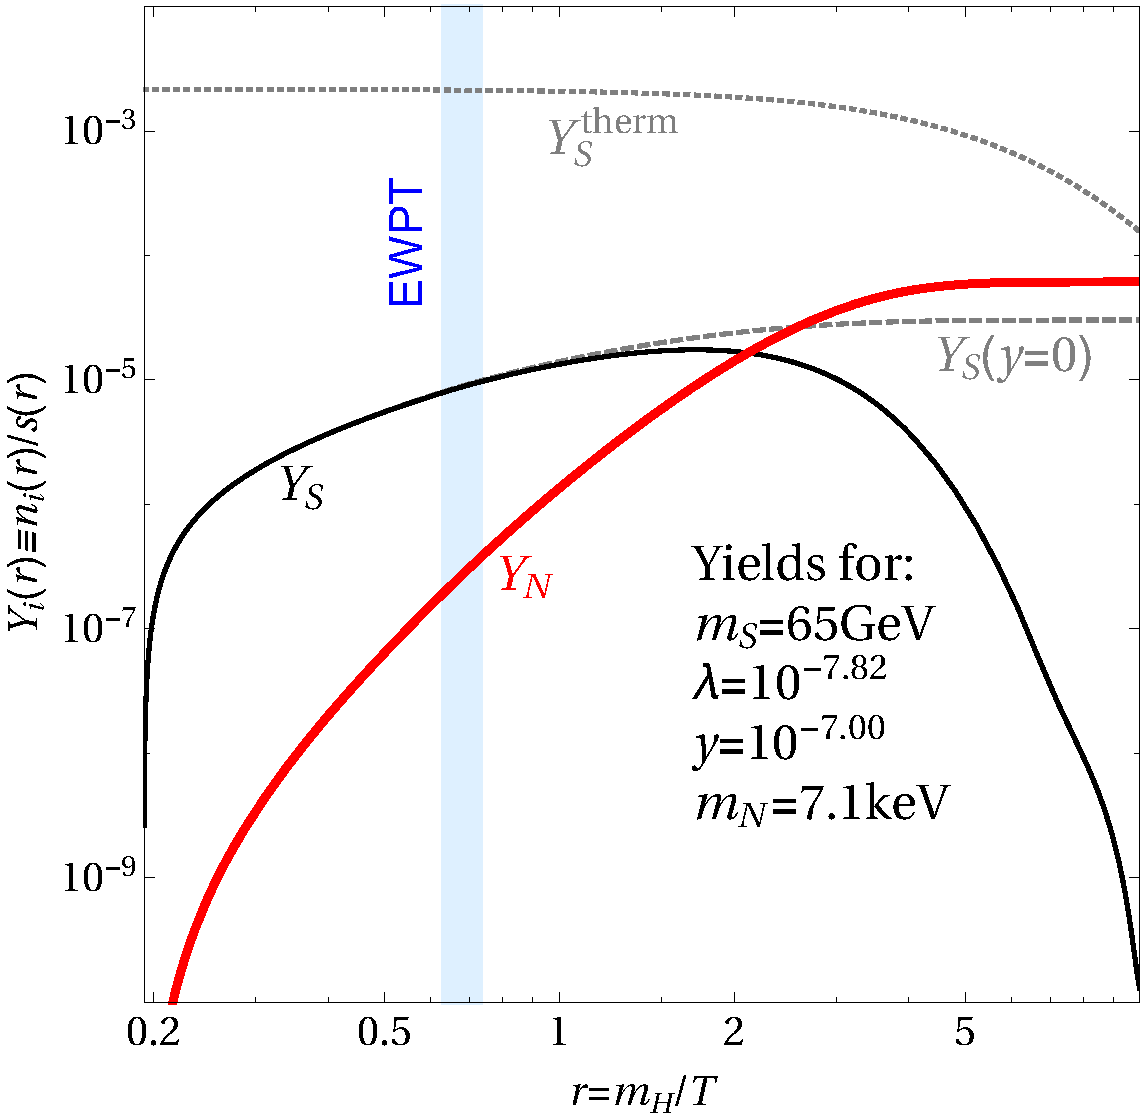
\includegraphics[width=7.9cm]{figures/yield65FIMP.pdf} & 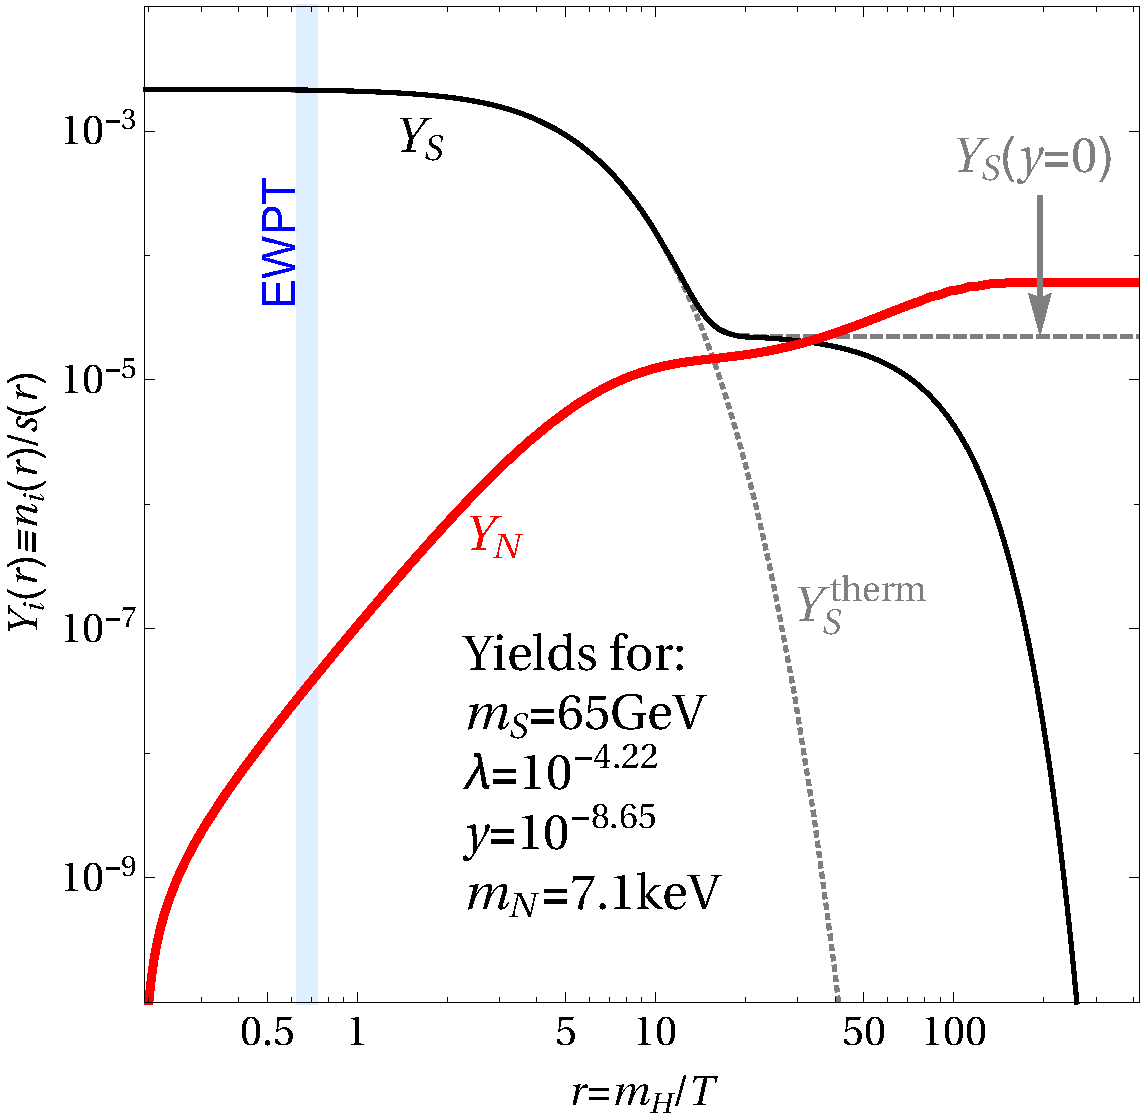
\includegraphics[width=7.9cm]{figures/yield65WIMP.pdf}\\
 \hspace{-1cm}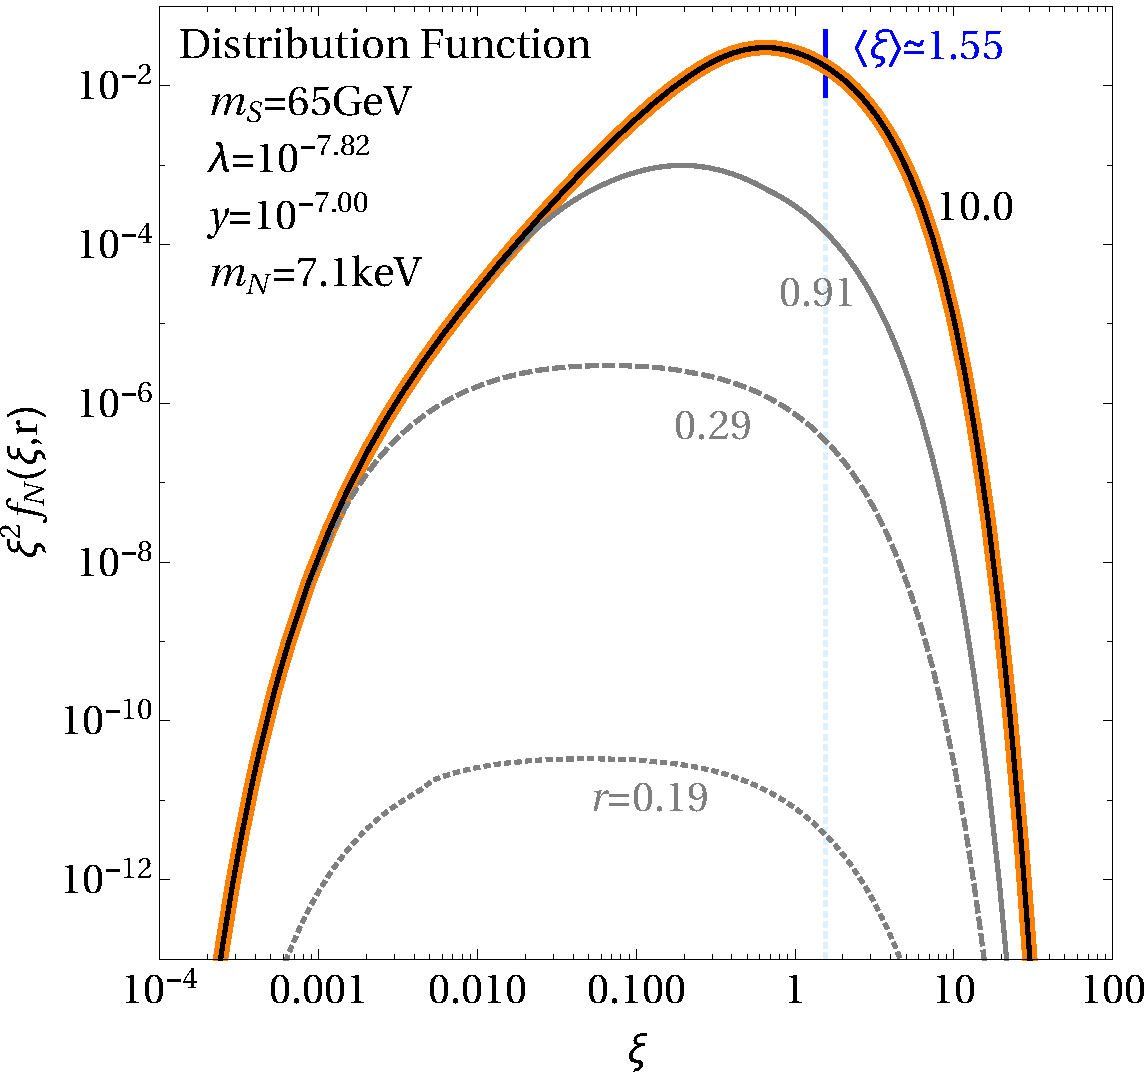
\includegraphics[width=8.3cm]{figures/snapshots65FIMP.pdf} & 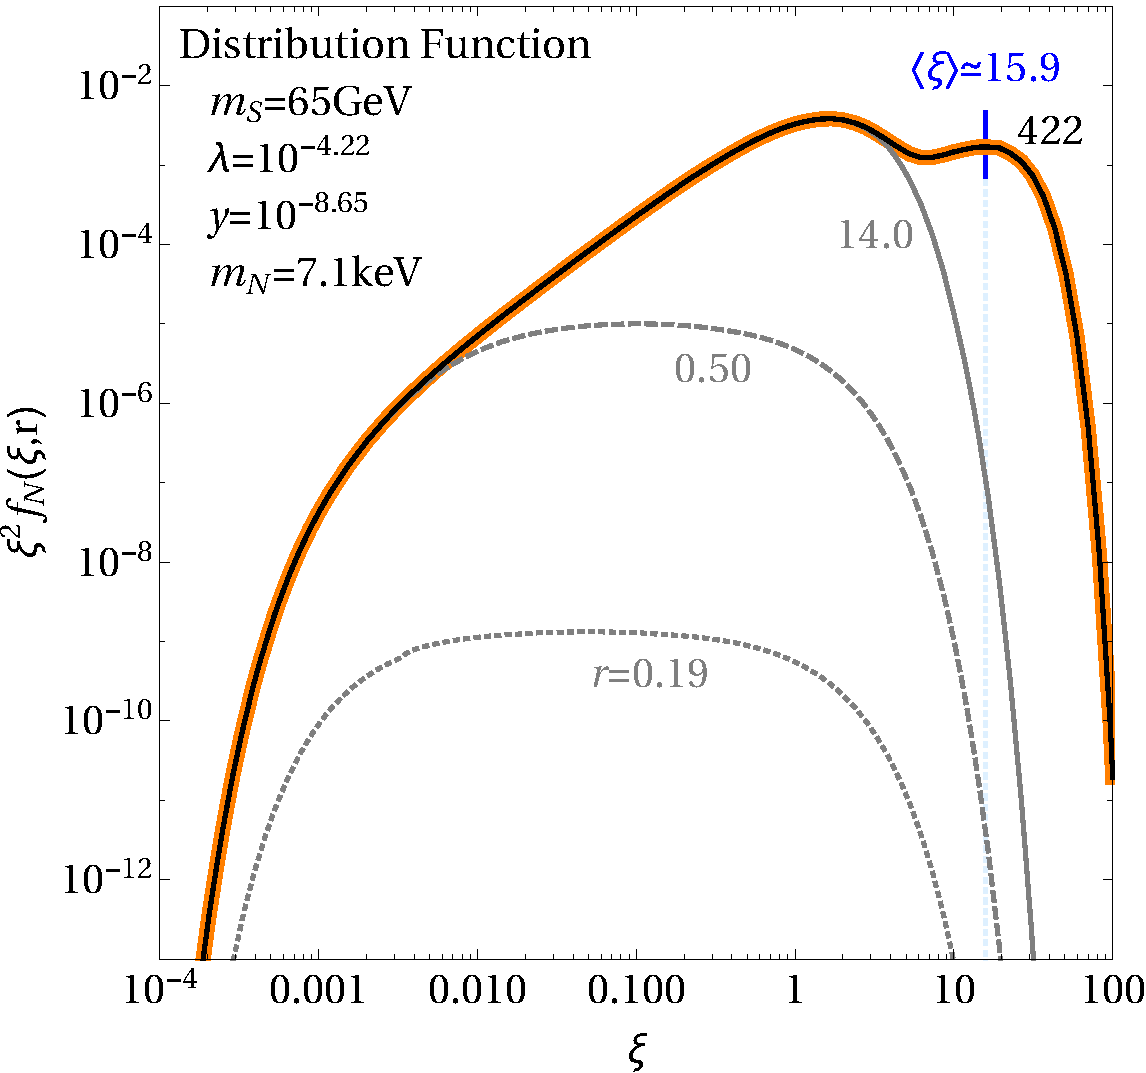
\includegraphics[width=8.3cm]{figures/snapshots65WIMP.pdf}
\end{tabular}
\caption{\label{fig:FIMP_WIMP_65}Example evolutions of the yield (\emph{top row}) and sterile neutrino distributions (\emph{bottom row}) for a scalar with a mass of $65$~GeV undergoing freeze-in (\emph{left}) or freeze-out (\emph{right}) before decaying into sterile neutrinos, for the two points marked in the left Fig.~\ref{fig:small_masses}.}
\end{figure}

As already anticipated, the lighter scalar ($m_S = 65$~GeV) freezes out \emph{earlier}, namely at $T\sim 17$~GeV, than the heavier one ($m_S = 100$~GeV), which does so at $T\sim 15$~GeV, cf.\ Fig.~\ref{fig:interaction_rates}. This may look surprising at first, since usually heavier particles tend to freeze out earlier due to the thermal suppression for non-relativistic particles. But the thermal suppression is similar for both cases, $e^{-65/100} \sim 0.5$, so that the actual interactions are decisive. Already at $T\sim 50$~GeV, all heavy bosons and the top are thermally suppressed, so that they cannot easily be produced anymore. However, a scalar with a mass of $100$~GeV can even at rest annihilate into both $W^+ W^-$ and $Z^0 Z^0$, while a lighter scalar cannot. Thus, the interaction rate of the heavier scalar is considerably larger, thereby keeping it in equilibrium significantly longer. It follows that the number density of the lighter scalar, and thus of the sterile neutrinos originating from its decay, is higher and hence must be compensated by a smaller sterile neutrino mass -- which is the origin of only small masses being allowed in the freeze-out region of the left Fig.~\ref{fig:small_masses}.

\begin{figure}[t]
\begin{tabular}{lr}\hspace{-1cm}
 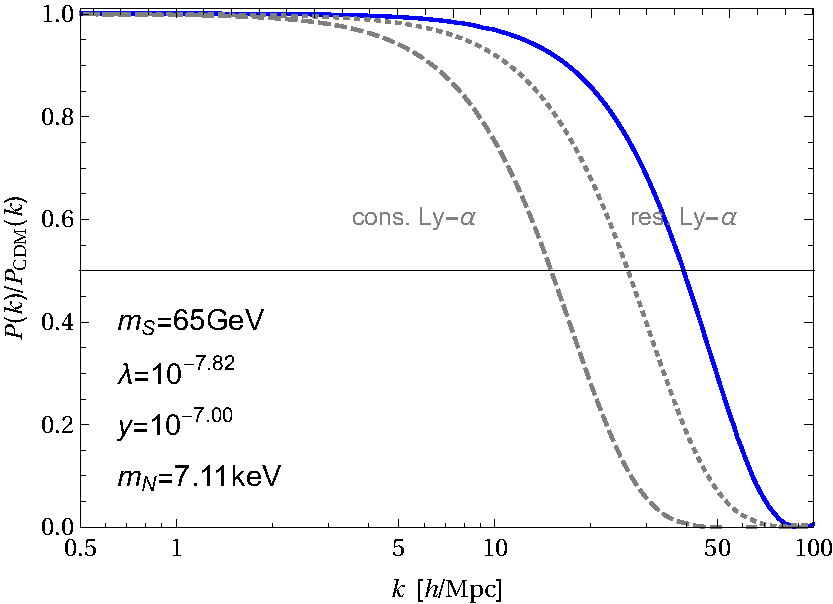
\includegraphics[width=8.3cm]{figures/SquaredTF_mS_65_FIMP.pdf} & 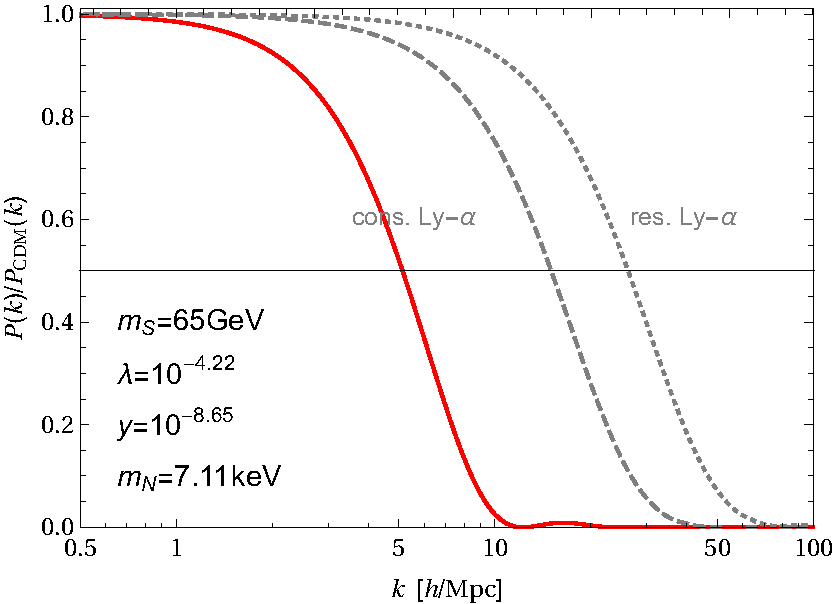
\includegraphics[width=8.3cm]{figures/SquaredTF_mS_65_WIMP.pdf}
\end{tabular}
\caption{\label{fig:TF_65}Example squared transfer functions for a scalar with a mass of $65$~GeV undergoing freeze-in (\emph{left}) or freeze-out (\emph{right}) before decaying into sterile neutrinos, for the two points marked in the left Fig.~\ref{fig:small_masses}.}
\end{figure}

Again, two example points are depicted in Fig.~\ref{fig:FIMP_WIMP_65}, with the order of the plots as in Fig.~\ref{fig:FIMP_WIMP_60}. It is clearly visible that, in the yields of the scalars, the effect of the EWPT is much less dramatic than for the very light scalars. In the resulting sterile neutrino spectra, the effect of the EWPT is thus much less pronounced, although little bumps can be spotted on the left sides of both spectra in the bottom row of the figure. Qualitatively, the course of the DM production is similar to case of very light scalars: again, if the scalar freezes in, it gradually decays into sterile neutrinos; if it freezes out, then it may decay either in or out of equilibrium, which a gradual transition between the two regimes. Note that, for the masses displayed, the comparison to Ref.~\cite{Adulpravitchai:2014xna} is in fact much more difficult. While the same scalar masses are used in that reference, we strongly suspect that paper to have a small error in the degrees of freedom of the Higgs field above the EWPT. While the Higgs field does possess four physical components in the unbroken phase, in Ref.~\cite{Adulpravitchai:2014xna}, only one seems to have been used. In other words, at high $T$, while the gauge boson contributions are switched off, the contributions of the would-be Goldstone bosons are \emph{not} switched on, as one would need to do. We will confirm this claim later in Sec.~\ref{sec:Results_large}, where it results in a factor of four between our results and those obtained in Ref.~\cite{Adulpravitchai:2014xna}. However, this factor is only close to four for very heavy scalar masses (even when taking into account the difference in the normalisation of $\lambda$, which also happens to be a factor of four), where the production almost entirely happens in regime~I. But for the comparatively light scalars treated in this subsection, the production is spread out over regimes~I and~II, cf.\ Fig.~\ref{fig:RegimeExampleCases}, such that a discrepancy by less than a factor of four but no perfect agreement can be expected. This is confirmed by our numerical results, making us confident that our treatment is the correct one for high temperatures.

The squared transfer functions (i.e., the ratios of the resulting linear power spectra to the CDM case) are depicted in Fig.~\ref{fig:TF_65}. As to be anticipated from the left Fig.~\ref{fig:small_masses}, the FIMP point is located in a blue region, and it should thus be perfectly allowed by all bounds. The WIMP point, in contrast, is in a region that is entirely red -- and it should thus correspond to DM that is by far too hot. Indeed, the squared transfer functions displayed in Fig.~\ref{fig:TF_65} confirm this conclusion. The whole curve of the FIMP case is in the allowed region, whereas the whole curve of the WIMP case is forbidden by far, even by the conservative bound. For such clear cases, an elaborate analysis would not even be necessary. Again we observe that, although both points feature a sterile neutrino mass of $7.1$~keV, the predictions for cosmic structure formation are different by far. This clearly illustrates that the DM mass itself is not at all a good way to discriminate between two different DM spectra, even if viewed at one and the same temperature.


%%%%%%%%%%%%%%%%%%%%%%%%%%%%%%%%%%%%%%%%%%%%%%%%%%%%%%%%%%
\subsection{\label{sec:Results_large}Heavy scalars: $\boldsymbol{m_h < m_S}$}
%%%%%%%%%%%%%%%%%%%%%%%%%%%%%%%%%%%%%%%%%%%%%%%%%%%%%%%%%%

Finally, the scalars may also be heavier than the Higgs, see Fig.~\ref{fig:large_masses}, which is the case that had already been discussed in our earlier reference~\cite{Merle:2015oja}. In this case, given that both freeze-in and freeze-out are correlated to the mass of the scalar, most of the production of scalars happens above the EWPT -- we basically remain in regime~I in Fig.~\ref{fig:RegimeExampleCases} during the whole production. Only for somewhat light scalar masses, such that $m_S/20 \lesssim T_{\rm EWPT}$, a small amount may be produced after the EWPT. However, for most of the production, only the simple 4-scalar interaction in the top row of Tab.~\ref{tab:RegimesFeynman} plays a role. In particular, one can greatly simplify the equations involved for $(m_h/m_S)^2 \ll 1$, see Ref.~\cite{Merle:2015oja} for details. As we can see from the central and right panels of Fig.~\ref{fig:interaction_rates}, it is in fact a good approximation to assume that the production of sterile neutrinos from very heavy scalars happens entirely before the EWPT -- thereby providing a clear justification of the assumptions made previously in~\cite{Merle:2015oja}.

\begin{figure}[t]
\begin{tabular}{lr}\hspace{-1cm}
 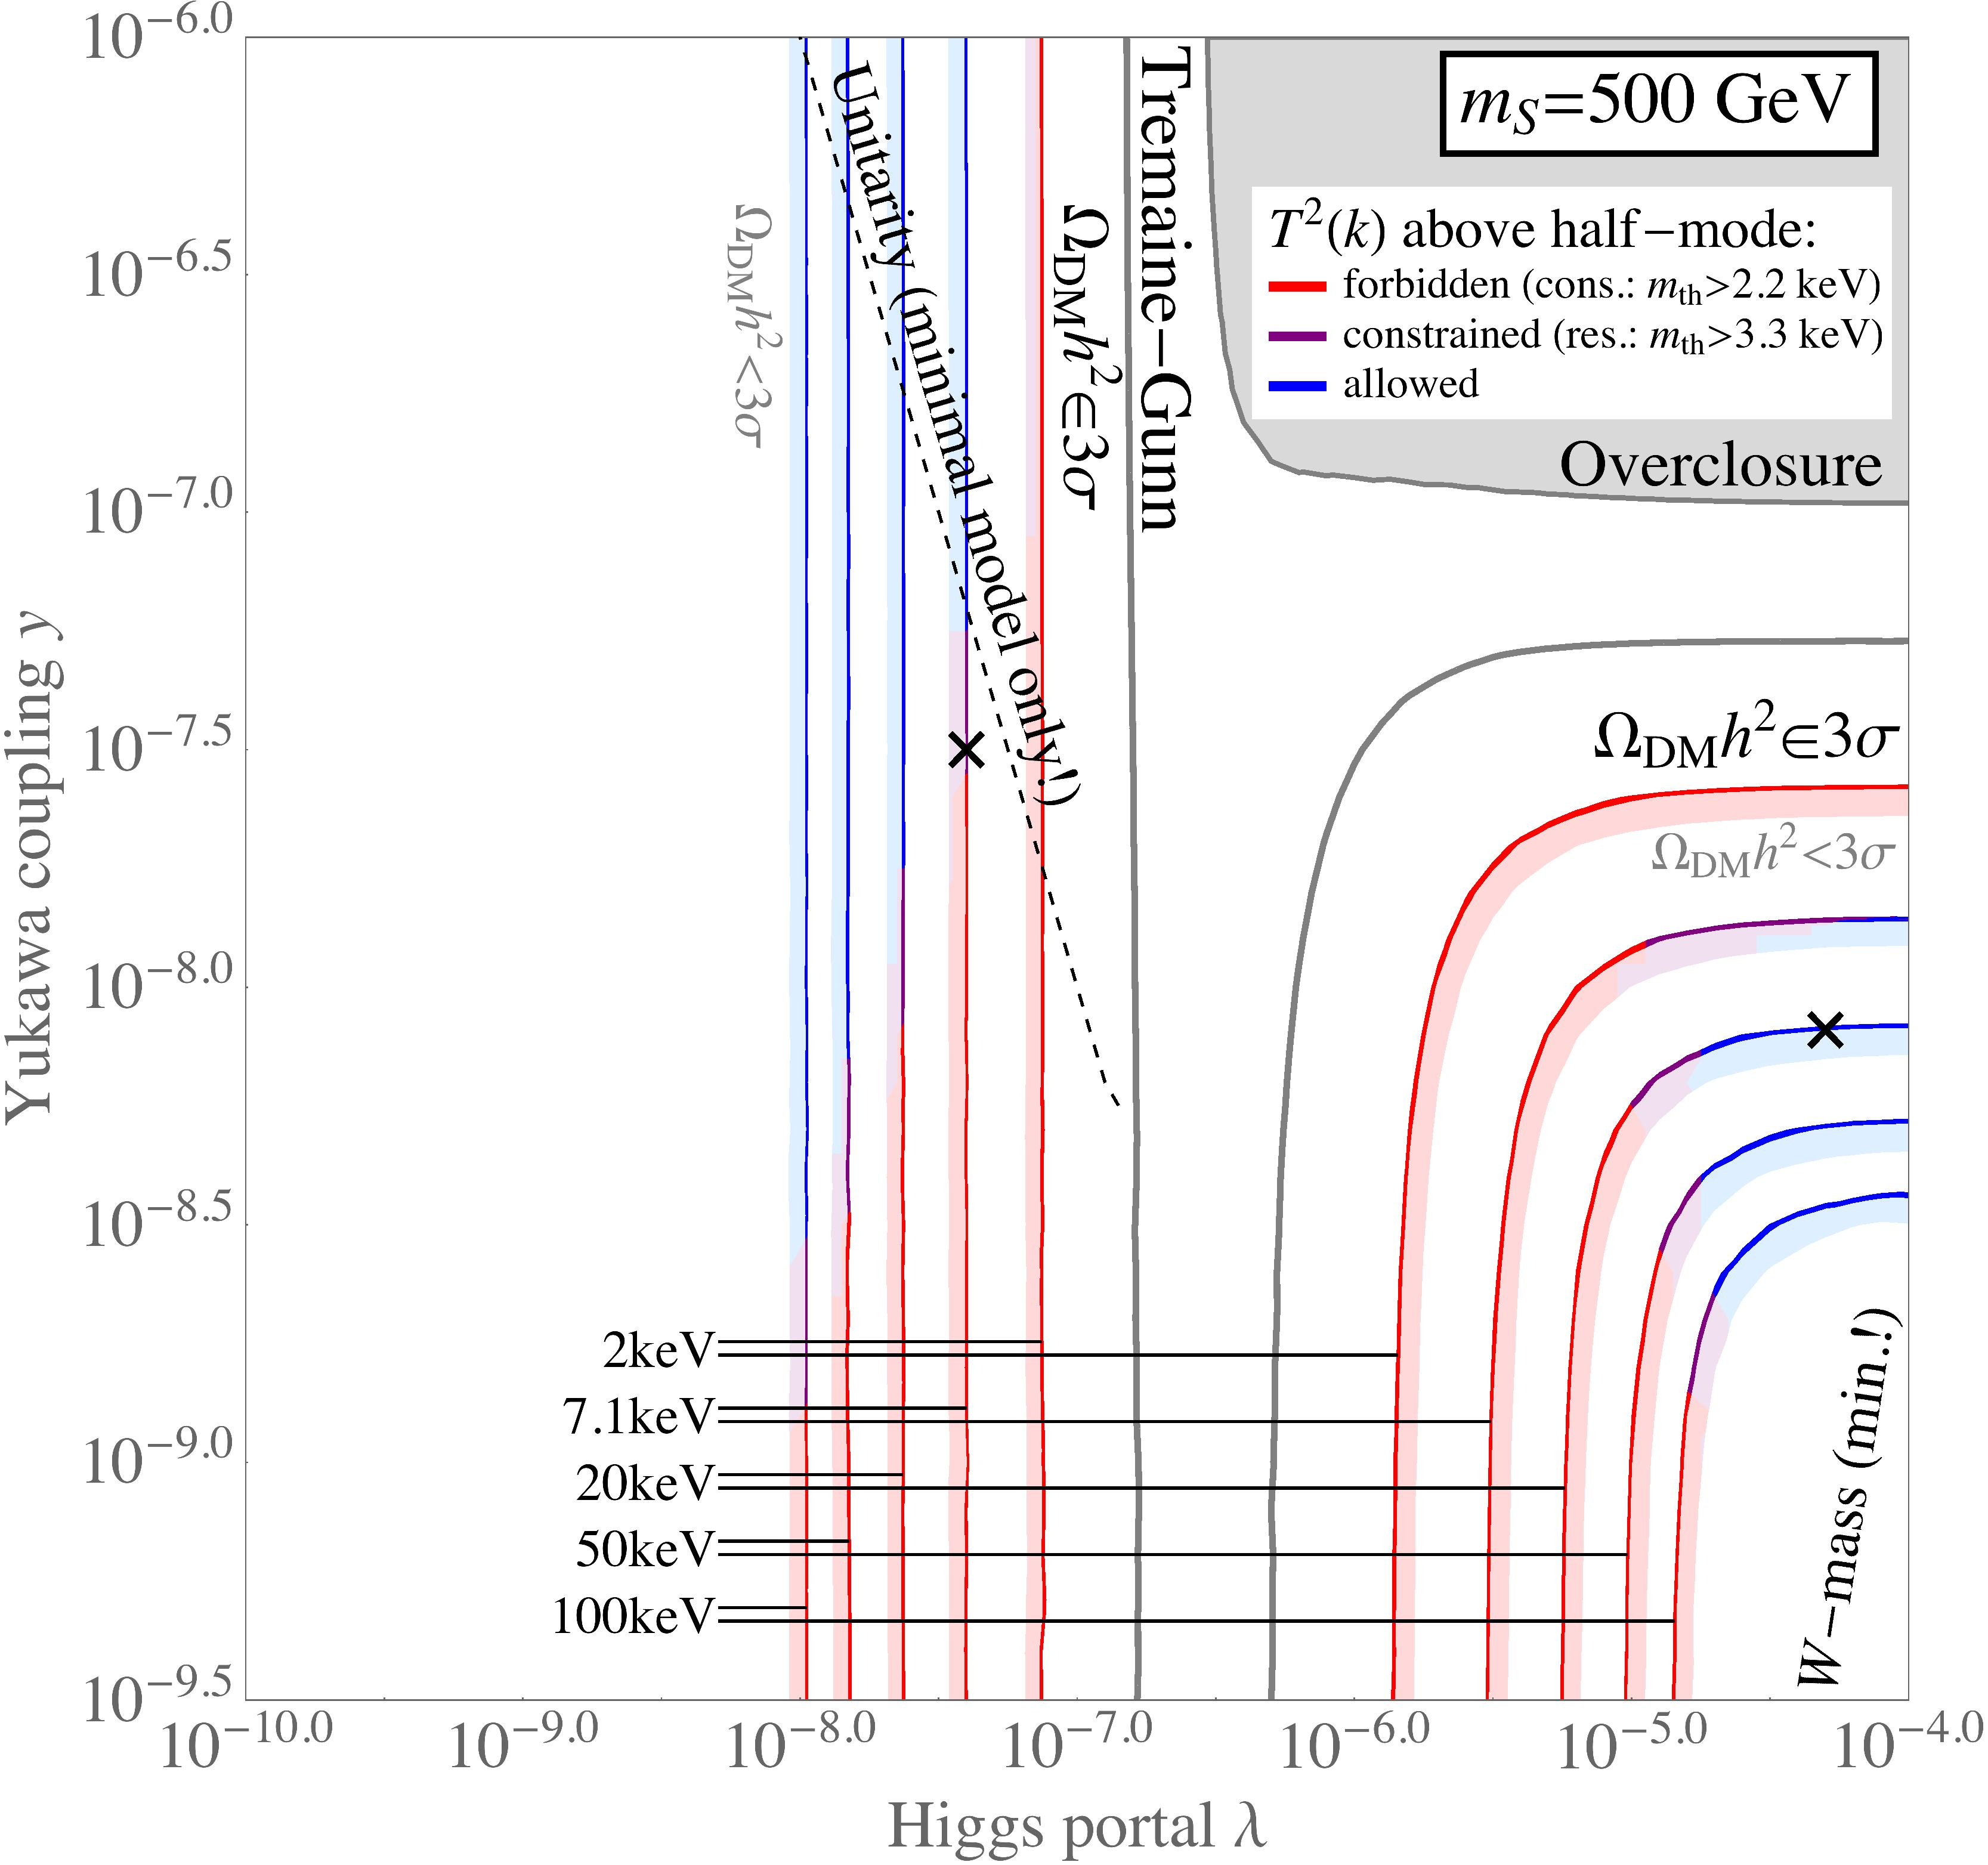
\includegraphics[width=8.3cm]{figures/HalfMode_500_until4.jpeg} & 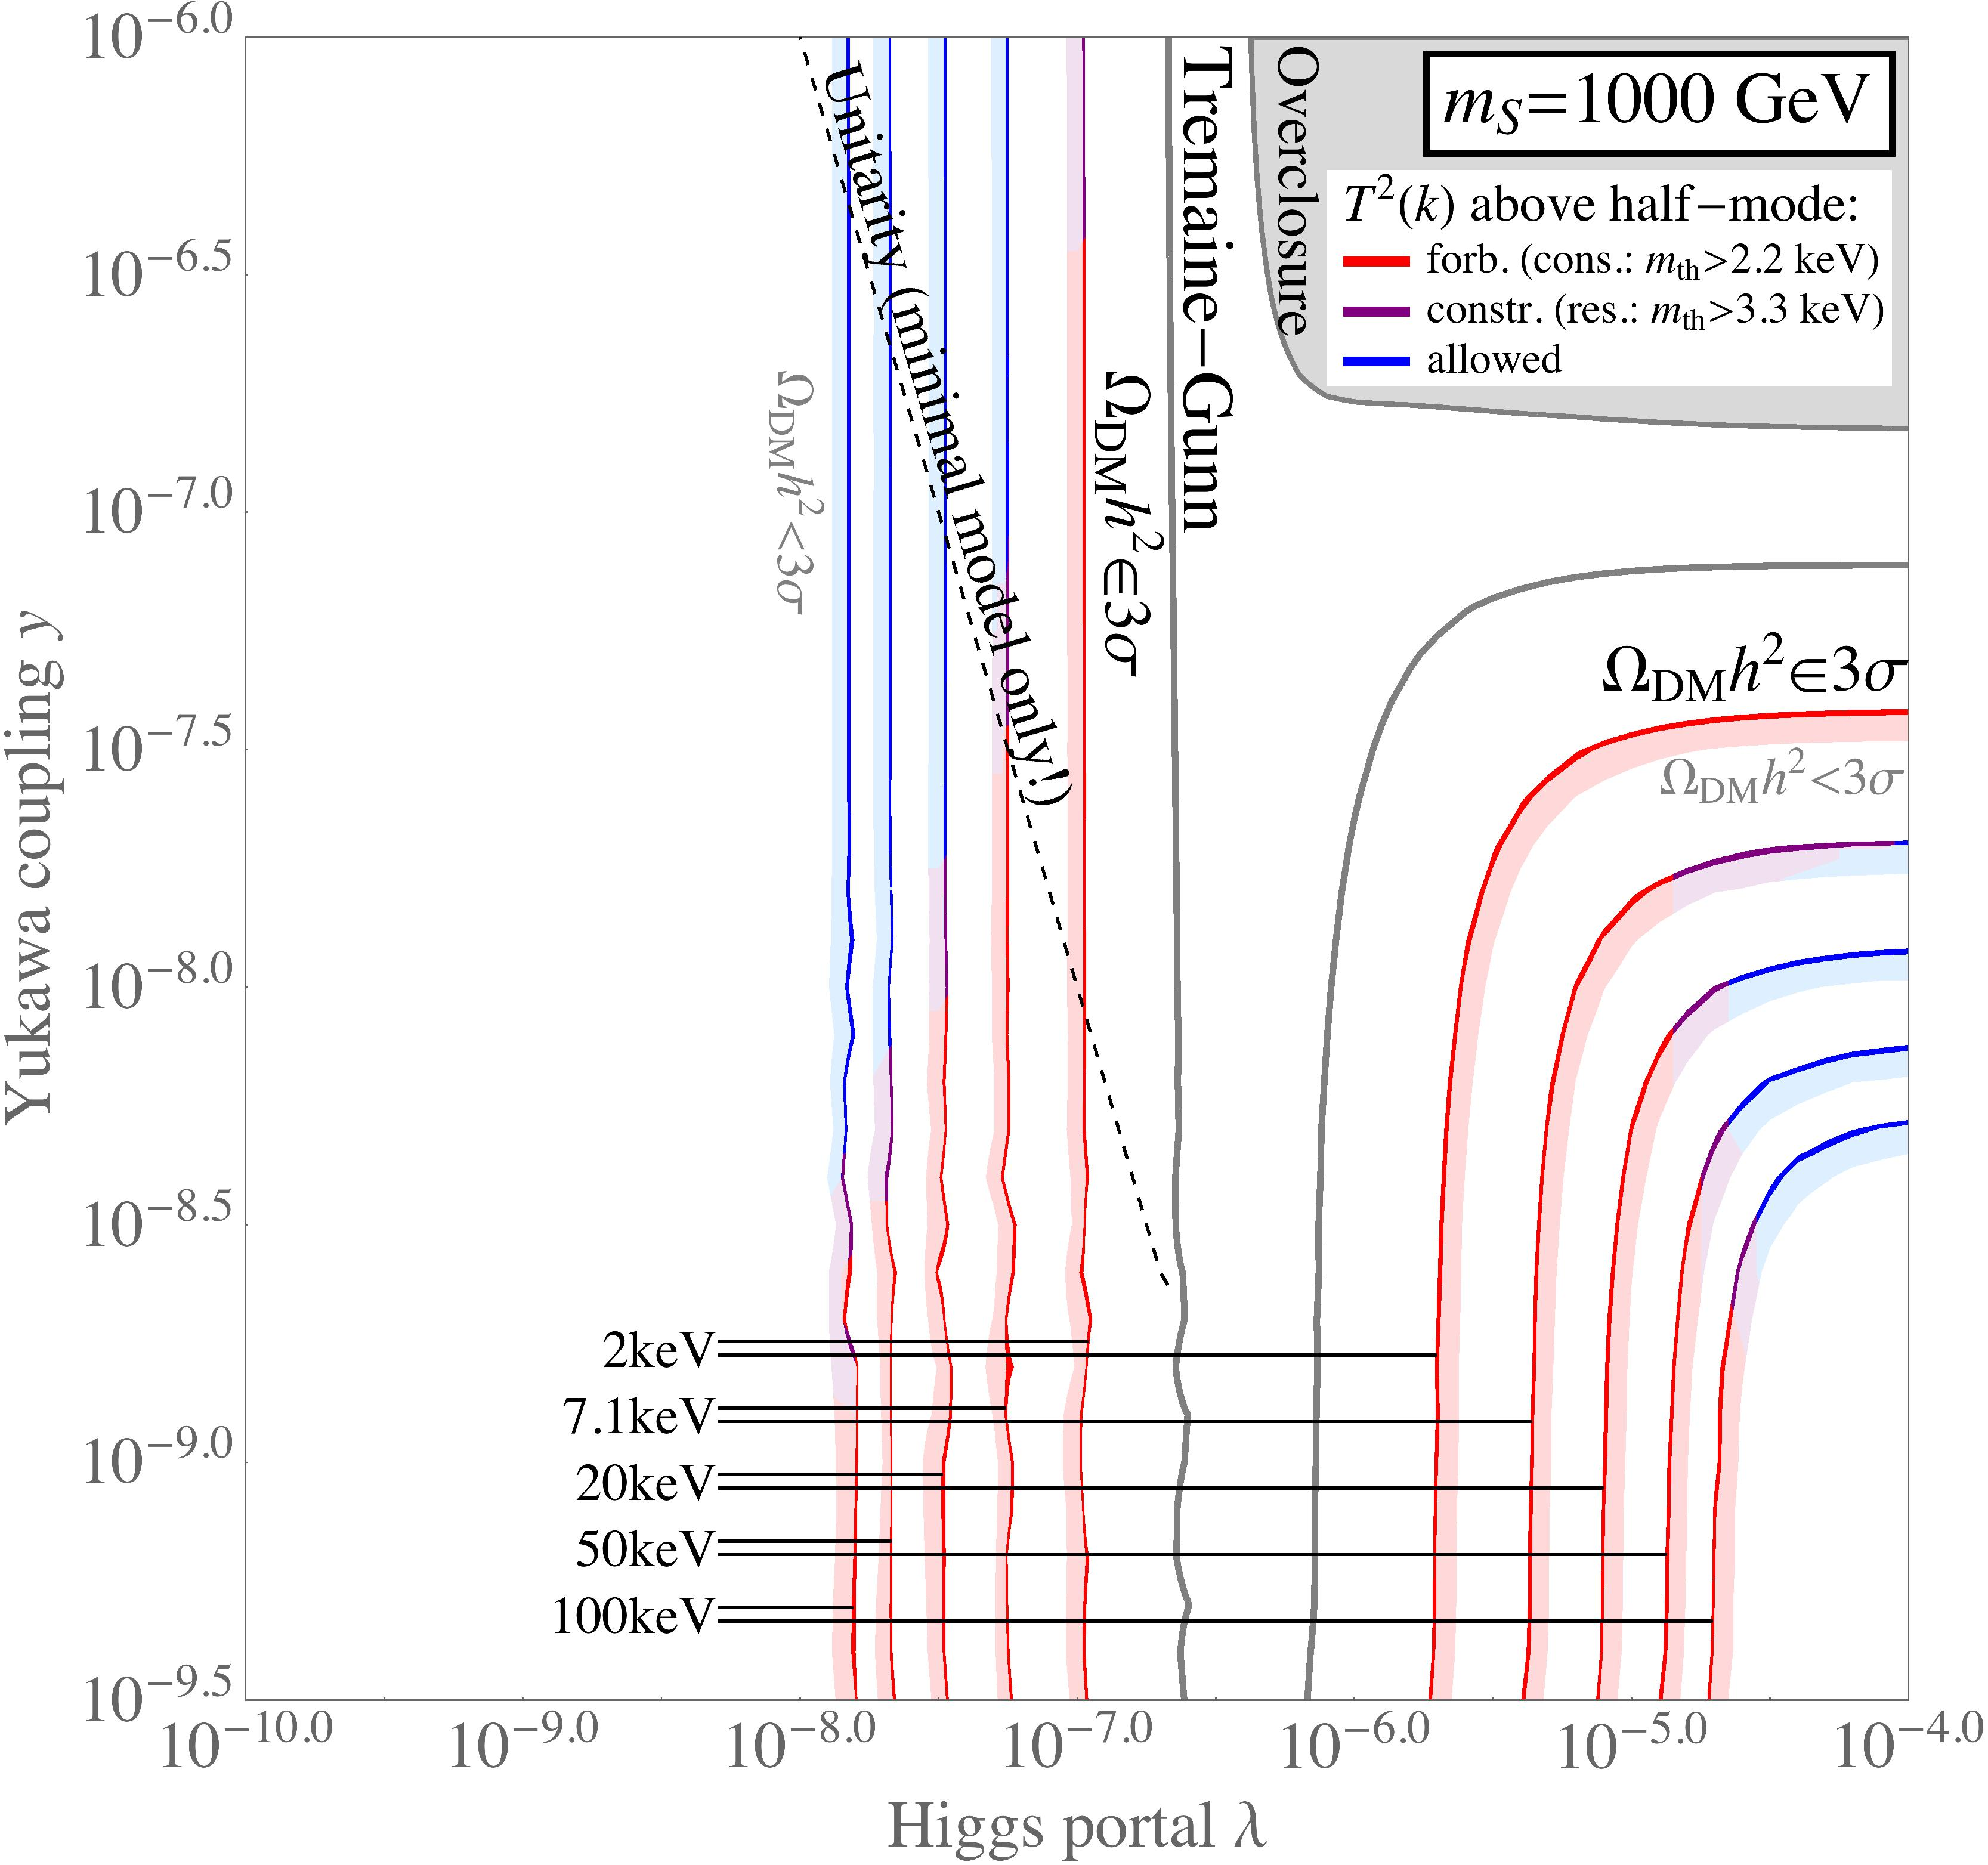
\includegraphics[width=8.3cm]{figures/HalfMode_1000_until4.jpeg}
\end{tabular}
\caption{\label{fig:large_masses}Abundance and constraints for large scalar masses, $m_h < m_S$. The crosses mark the points displayed explicitly in Fig.~\ref{fig:FIMP_WIMP_500}.}
\end{figure}

Understanding the results for this case is somewhat less subtle than for the previous two. Comparing the two plots depicted in Fig.~\ref{fig:large_masses}, one can see that there are no overly drastic changes. The reason is that, as argued in Ref.~\cite{Merle:2015oja}, there is a trade-off between a heavier scalar and an earlier decay: a larger scalar mass means that the production of scalars ceases at higher temperatures. In the freeze-in case, this indicates a lower overall production, which is what the vertical lines in that regime slightly shift to the right when going from $m_S = 500$~GeV to $1000$~GeV. However, given that no new production channels open up while staying in regime~I, the change is rather mild. In the other limiting case, where the scalar freezes out, a larger scalar mass means a larger abundance for the case where the scalar decays mainly after freeze-out (i.e., the vertical lines on the bottom right of the plots). Thus, these vertical lines should slightly shift to the left to compensate for that, which they indeed do, as visible in the plots. For the horizontal parts of the lines, where the scalar decays while in equilibrium, however, freezing out earlier means less sterile neutrinos unless this is compensated by a larger decay rate: thus, these lines should shift to slightly larger values of the Yukawa coupling $y$ when going from $m_S = 500$~GeV to $1000$~GeV, which is just what is visible in the plot.

\begin{figure}[t!]
\begin{tabular}{cc}
 \hspace{-1cm}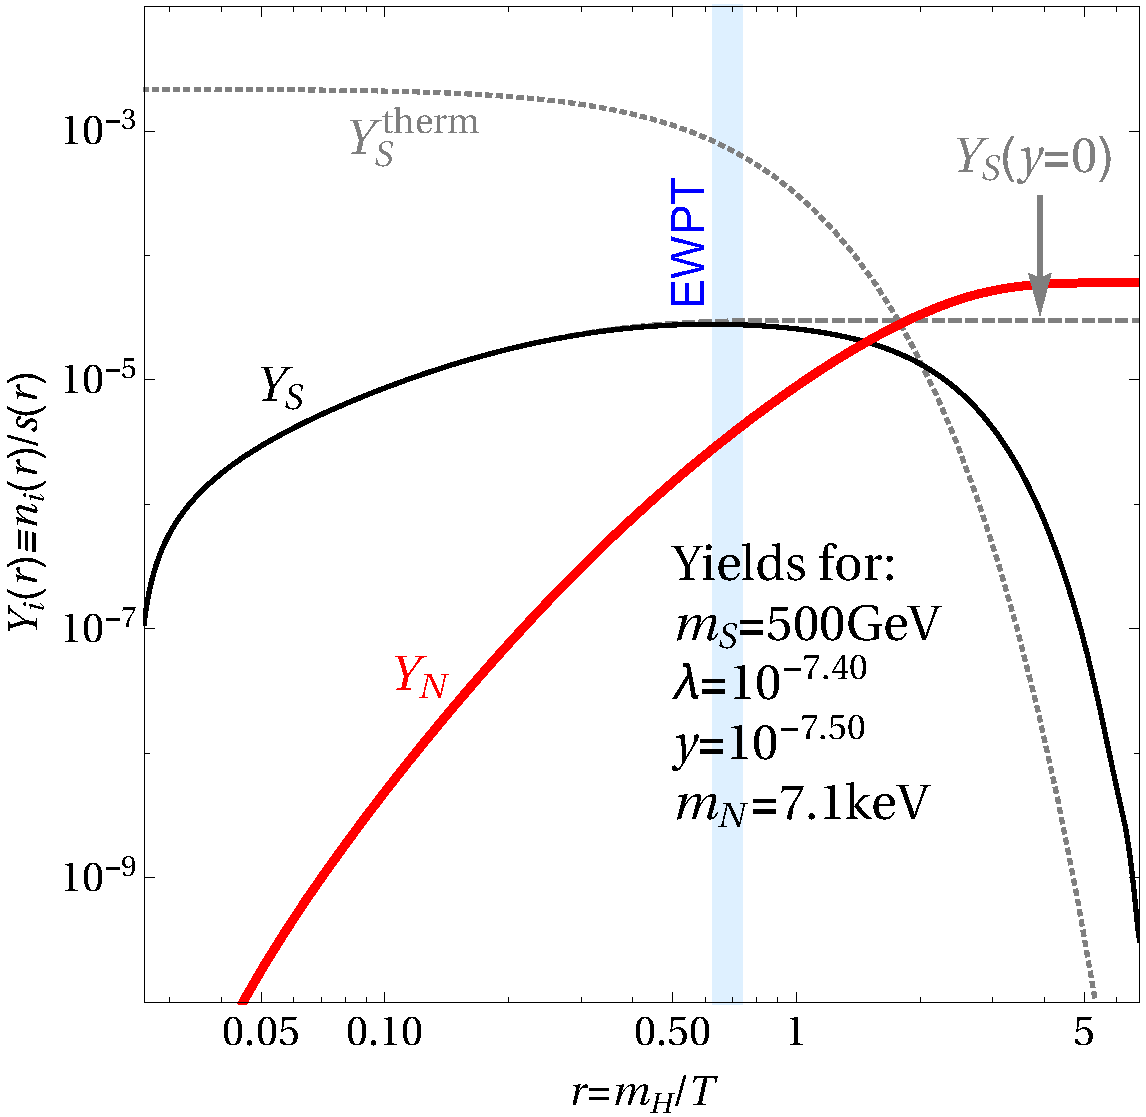
\includegraphics[width=7.9cm]{figures/yield500FIMP.pdf} & 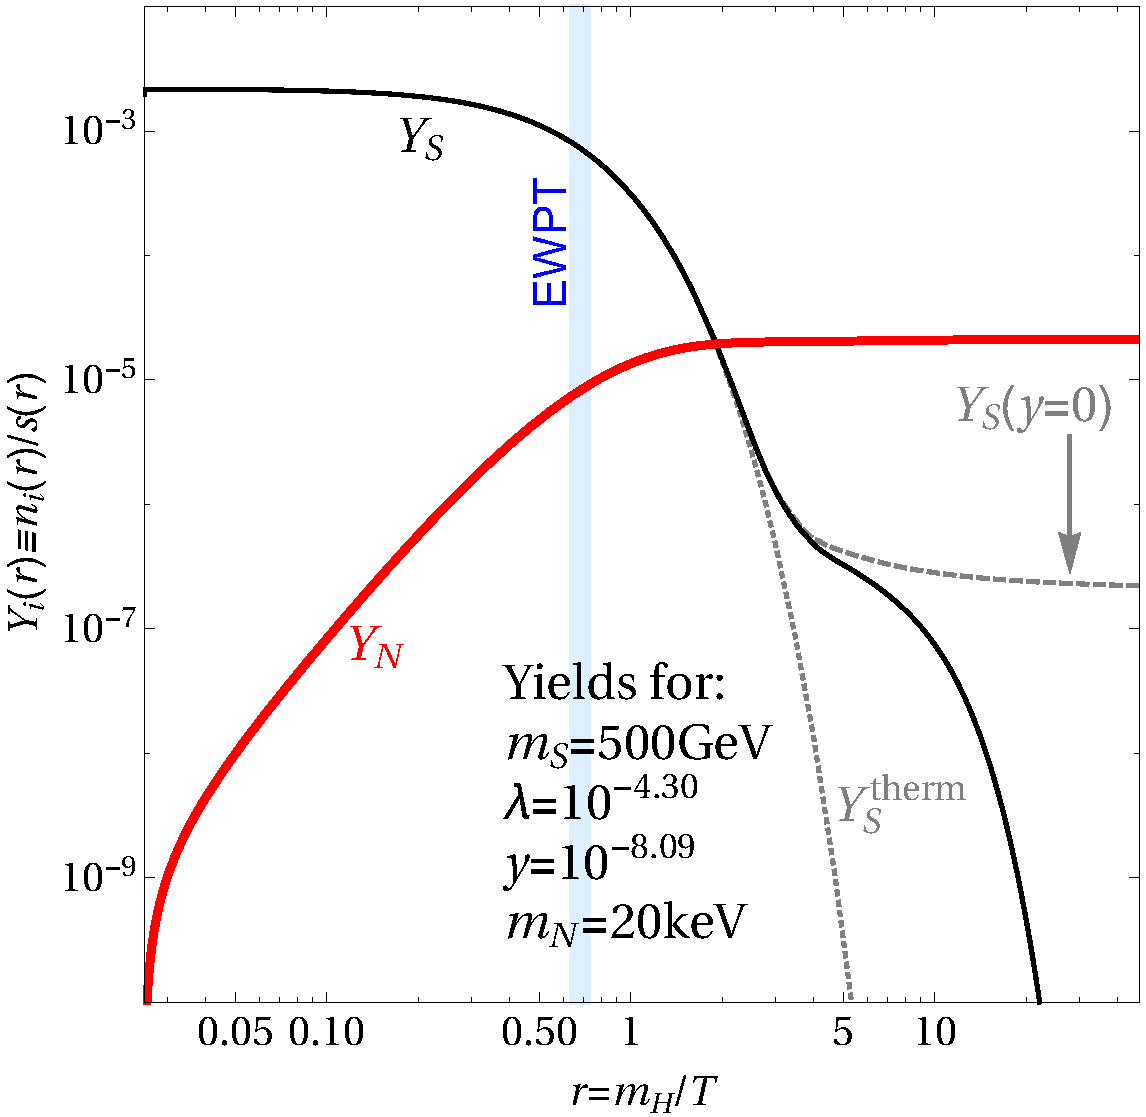
\includegraphics[width=7.9cm]{figures/yield500WIMP.pdf}\\
 \hspace{-1cm}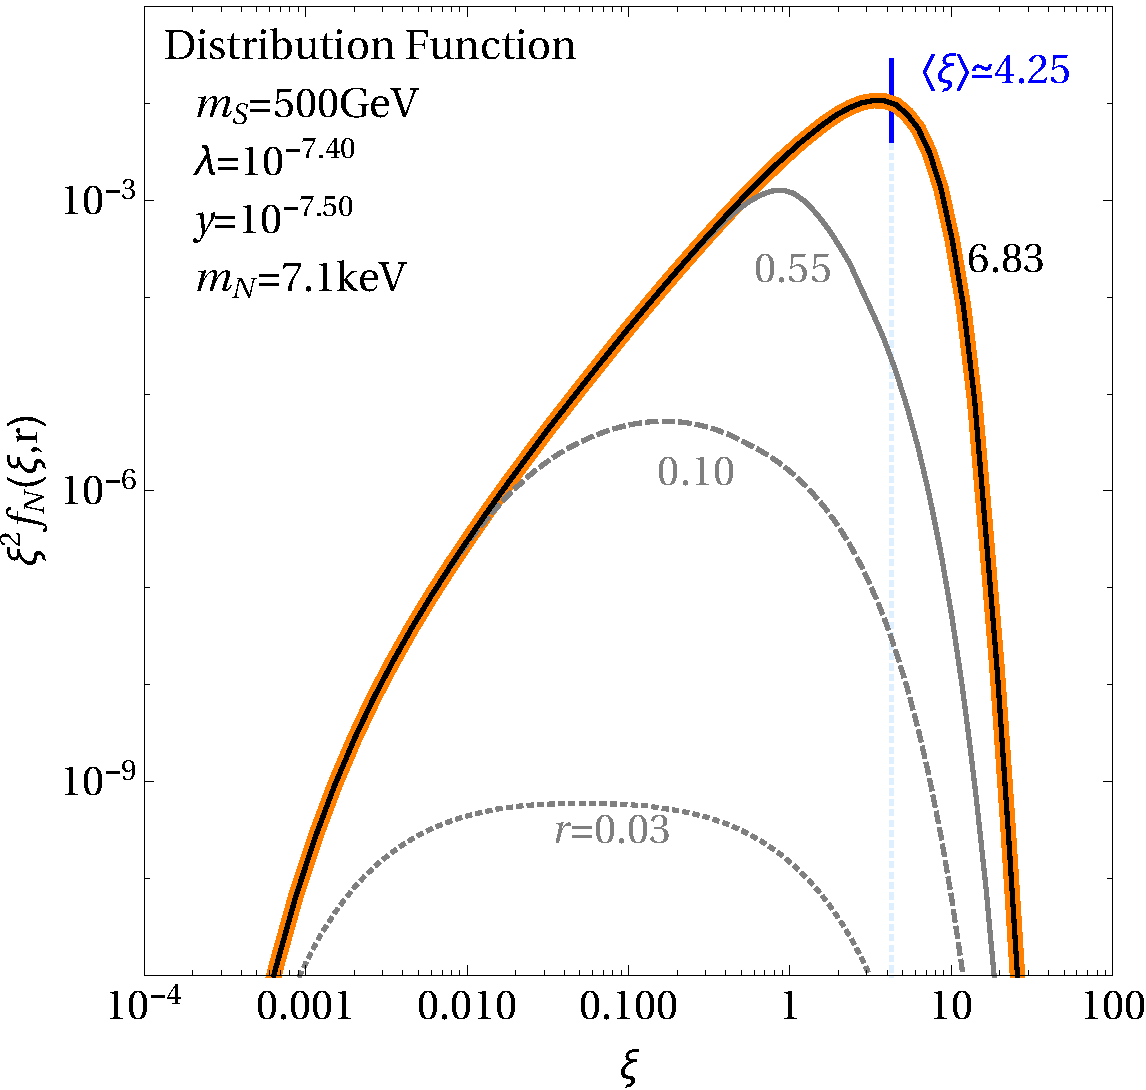
\includegraphics[width=8.3cm]{figures/snapshots500FIMP.pdf} & 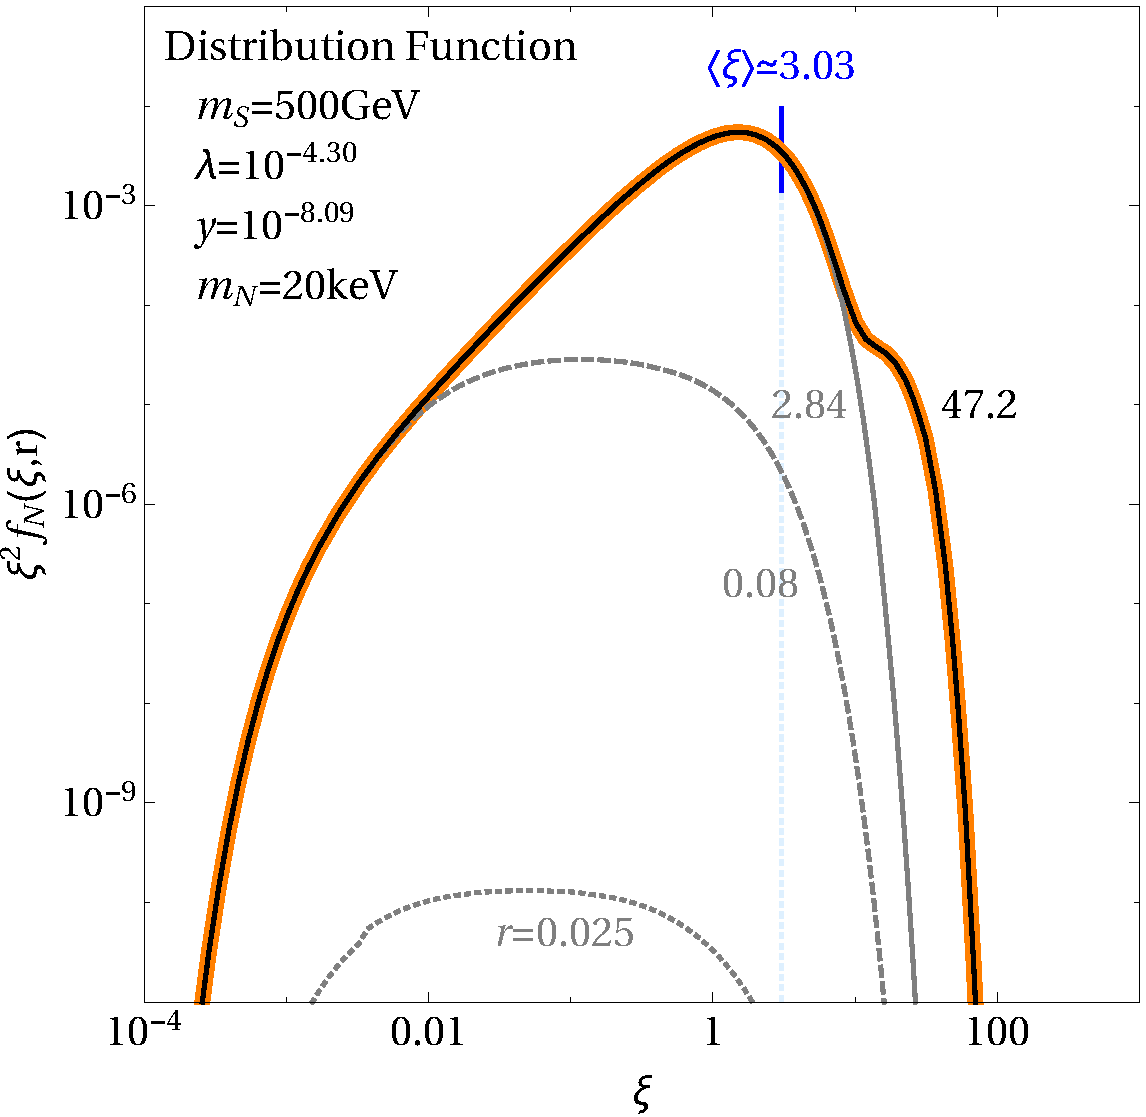
\includegraphics[width=8.3cm]{figures/snapshots500WIMP.pdf}
\end{tabular}
\caption{\label{fig:FIMP_WIMP_500}Example evolutions of the yield (\emph{top row}) and sterile neutrino distributions (\emph{bottom row}) for a scalar with a mass of $500$~GeV undergoing freeze-in (\emph{left}) or freeze-out (\emph{right}) before decaying into sterile neutrinos, for the two points marked in the left Fig.~\ref{fig:large_masses}.}
\end{figure}

Two representative example evolutions of the yield can be seen in the upper row of Fig.~\ref{fig:FIMP_WIMP_500}, both for the scalar freezing in (\emph{left}) or out (\emph{right}). Just as before, in the FIMP case, the scalar is gradually produced but never reaches a thermal abundance before freezing in (while constantly decaying), whereas for the WIMP-case it quickly thermalises before freezing out. Also here, the decay can happen earlier or later, depending on the value of $y$. As already hinted in Sec.~\ref{sec:Results_Light}, we expect a factor four difference compared to the results obtained in Ref.~\cite{Adulpravitchai:2014xna}, as DM production happens nearly completely in regime~I. This approximation is best for very large scalar masses, however, the most extreme case discussed in~\cite{Adulpravitchai:2014xna} involves a scalar with $m_S = 500$~GeV. Taking the same couplings as in the reference and taking into account the different normalisation of $\lambda$, the discrepancy obtained numerically is already larger than a factor of three, and should converge to four for even larger scalar masses (which we however cannot explicitly check, given the absence of this case in~\cite{Adulpravitchai:2014xna}). Yet, given that no distribution functions had been computed in Ref.~\cite{Adulpravitchai:2014xna}, their results can be rectified by simply including the missing factor.

\begin{figure}[t]
\begin{tabular}{lr}\hspace{-1cm}
 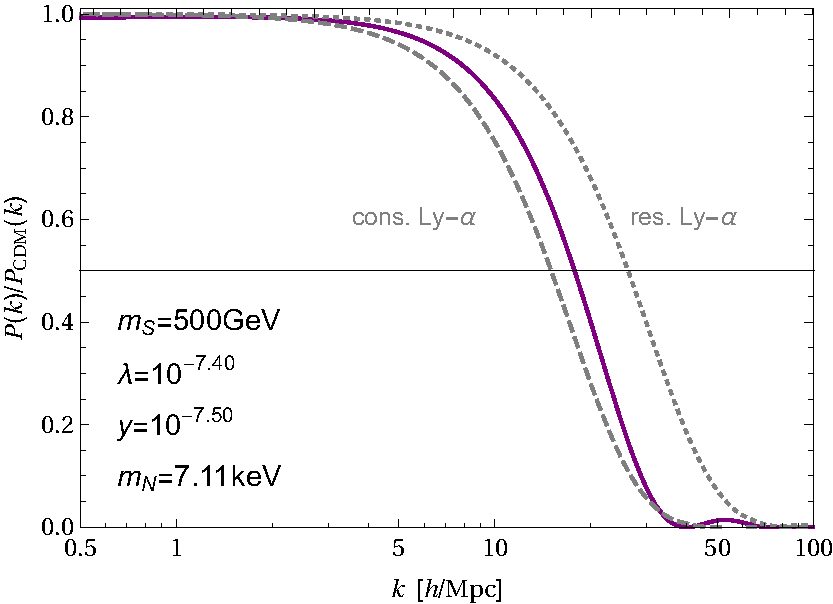
\includegraphics[width=8.3cm]{figures/SquaredTF_mS_500_FIMP.pdf} & 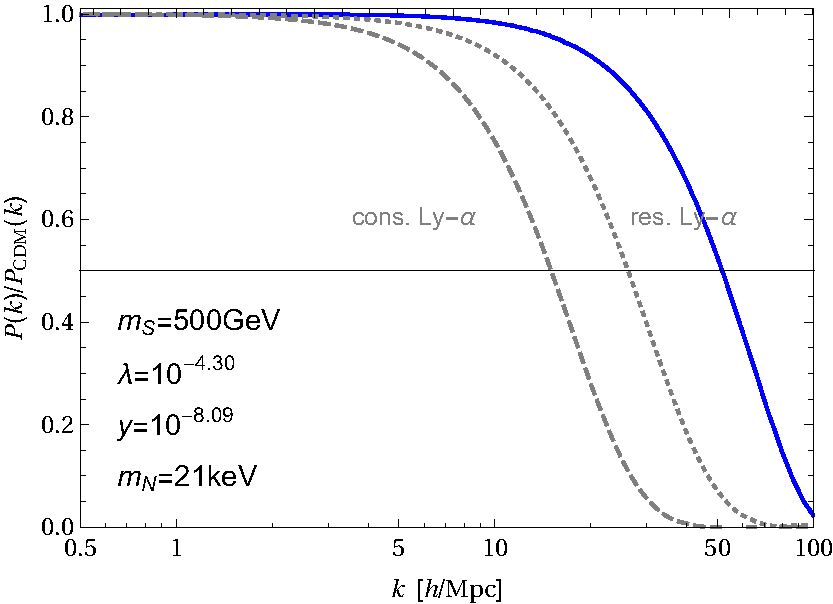
\includegraphics[width=8.3cm]{figures/SquaredTF_mS_500_WIMP.pdf}
\end{tabular}
\caption{\label{fig:TF_500}Example squared transfer functions for a scalar with a mass of $500$~GeV undergoing freeze-in (\emph{left}) or freeze-out (\emph{right}) before decaying into sterile neutrinos, for the two points marked in the left Fig.~\ref{fig:large_masses}.}
\end{figure}

The corresponding evolutions of the distribution functions are depicted on the bottom row of Fig.~\ref{fig:FIMP_WIMP_500}, with similar characteristics as for smaller masses. One big difference, though, is that the DM production is finished much earlier, which comes from heavier scalars decaying faster. This allows more time to redshift, but it is compensated to some extend by a larger initial velocity.

In what concerns structure formation, however, these shifts do not change very much. In the freeze-out case, while the sterile neutrinos are produced by a heavier scalar and are thus faster, they are also produced earlier (since the decay rate of the scalar is proportional to its mass), so that hardly any change in the colouring can be seen for the freeze-in case when comparing the two plots in Fig.~\ref{fig:large_masses}. For the case of the scalar freezing out,  only the in-equilibrium decays are phenomenologically relevant, as the late decays in any case produce too ``hot'' Dark Matter. However, for scalars decaying while in equilibrium, a larger mass translates into larger Yukawa couplings and thus into earlier decays so that, again, the resulting sterile neutrinos have a larger momentum at production but they have also more time to redshift, such that the prediction for structure formation remains basically unaffected -- hence the similarity between both plots. Note that, for large scalar masses, none of the ``kink'' regions on the bottom right of the plot is allowed, which would correspond to a double peak structure in the sterile neutrino's momentum distribution function (due to nearly equal contributions from the decays before and after freeze-out of the scalar) -- such distributions do exist but they are already peaking into the region of the restrictive Lyman-$\alpha$ bounds. This result is consistent with the findings from Ref.~\cite{Merle:2015oja}, which analysed just that case, and it is also backed up by the example squared transfer functions, cf.\ Fig.~\ref{fig:TF_500}.
